\documentclass[11pt,a4paper, onecolumn]{article}

\usepackage[a4paper,margin=15mm]{geometry}
\usepackage{amsmath,amssymb,amsfonts,bm}
\usepackage{graphicx}
\usepackage{subcaption}
\usepackage{booktabs}
\usepackage{multirow}
\usepackage{array}
\usepackage{float}
\usepackage{placeins}
\usepackage{hyperref}
\usepackage{xcolor}
\usepackage{enumitem}
\usepackage{caption}
\usepackage{pdfpages}
\usepackage{fancyhdr}
\pagestyle{fancy}
\fancyhead[L]{3875B}
\fancyhead[R]{4C11 Assignment 3}

\hypersetup{
    colorlinks=true,
    linkcolor=blue!60!black,
    citecolor=blue!60!black,
    urlcolor=blue!60!black
}

\graphicspath{{figures/}{figures/optuna/}}

\newcommand{\epsbar}{\bar{\epsilon}}
\newcommand{\sigbar}{\bar{\sigma}}
\newcommand{\dt}{\Delta t}
\newcommand{\R}{\mathbb{R}}

\title{\textbf{4C11 Coursework 3 Report} \\ Recurrent Neural Operator - one dimensional visco-plasticity}
\author{3875B}
\date{March 31, 2026}

\begin{document}
\maketitle

\section{Introduction}

This report studies the unit-cell problem posed in the coursework brief: a one-dimensional three-phase viscoelastic composite driven by a prescribed macroscopic strain history. The practical aim is to learn a macroscopic constitutive model from data, while the scientific aim is to understand how much hidden state is actually required to represent the material memory. This was done using various types of recurrent neural operators (RNO).

The most direct answer to part (a) is that the macroscopic constitutive model takes the applied macroscopic strain history as input and returns the macroscopic stress history as output. In operator form,
\begin{equation}
\sigbar(t)=\mathcal{G}\!\left(\epsbar_{[0,t]}\right),
\label{eq:macro_operator}
\end{equation}
where $\epsbar_{[0,t]}$ denotes the strain history from time $0$ to time $t$. In discrete form, consistent with the supplied dataset,
\begin{equation}
\left\{\epsbar_n\right\}_{n=0}^{1000}\mapsto \left\{\sigbar_n\right\}_{n=0}^{1000}.
\label{eq:discrete_operator}
\end{equation}
The dataset contains only macroscopic strain and stress histories, so the task is not to identify microscopic fields or microscopic parameters directly. In particular, the report does \emph{not} treat the microscopic Young's moduli and viscosities of the three phases as supervised outputs, as these variables are unknown. Instead, it learns a homogenised history-dependent constitutive law.

One important modelling note concerns the constitutive equation stated in the brief. The printed form uses a viscous term proportional to $\partial u/\partial t$, but for a Kelvin--Voigt-type constitutive law the physically consistent interpretation is a strain-rate term proportional to $\partial \epsilon/\partial t$. The implementation and the analysis therefore interpret the viscous response as strain-rate based, consistent with standard one-dimensional linear viscoelasticity.

The report is organised as a comparative investigation rather than a single-model demonstration. First, a data-driven architecture search is carried out over standard recurrent cells: vanilla RNN, GRU, and LSTM. Second, the hidden-variable question from part (c) is revisited using more physically structured recurrent neural operators inspired by the coursework skeleton and by the state-space formulation proposed by Liu et al.~\cite{Liu_2023}. This second stage is necessary because the first hidden-size sweep did not reveal a single dramatic threshold, and understanding \emph{why} that happened turns out to be one of the main results of the project.

\section{Problem Setup, Data and Method Overview}

\subsection{Problem Setup and Data}

To restate from the coursework brief, the microscopic unit-cell problem is governed by kinematics, equilibrium, and a linear elastic-viscous constitutive law. In one dimension,
\begin{equation}
\epsilon(x,t)=\frac{\partial u(x,t)}{\partial x},
\label{eq:kinematic_relation}
\end{equation}
\begin{equation}
\frac{\partial \sigma(x,t)}{\partial x}=0,
\label{eq:equilibrium_relation}
\end{equation}
and, phasewise,
\begin{equation}
\sigma_i(t)=E_i\,\epsilon_i(t)+\eta_i\,\dot{\epsilon}_i(t),
\label{eq:kelvin_voigt_phase}
\end{equation}
where $E_i$ and $\eta_i$ are piecewise-constant material parameters for the three phases. Equation~\eqref{eq:equilibrium_relation} implies that the stress is uniform across the unit cell, while the phase strains remain distinct. For a three-phase series composite,
\begin{equation}
\sigbar(t)=\sigma_1(t)=\sigma_2(t)=\sigma_3(t),
\label{eq:uniform_stress}
\end{equation}
\begin{equation}
\epsbar(t)=f_1\epsilon_1(t)+f_2\epsilon_2(t)+f_3\epsilon_3(t),
\label{eq:macro_strain_average}
\end{equation}
with phase fractions $f_1+f_2+f_3=1$. Since each $\epsilon_i(t)$ evolves in time, the macroscopic law is history dependent even though each phase is linearly viscoelastic.

The dataset contains $400$ paired strain and stress histories, each sampled at $1001$ time points. A deterministic split (with seed $20260328$) was used throughout: $280$ training samples, $60$ validation samples, and $60$ test samples, based on a commonly used 70/15/15 percentage split. The time step is
\begin{equation}
\dt=\frac{1}{1000}=10^{-3}.
\label{eq:dt_definition}
\end{equation}
Train-only min--max scaling to the interval $[-1,1]$ was used for both input and output histories to prevent information leakage from the validation and test sets, and to normalise the data for the neural network.

\begin{table}[t]
\centering
\caption{Dataset and preprocessing summary used throughout the study.}
\label{tab:data_summary}
\begin{tabular}{ll}
\toprule
Quantity & Value \\
\midrule
Total sequences & $400$ \\
Time steps per sequence & $1001$ \\
Training / validation / test split & $280/60/60$ \\
Time step $\dt$ & $10^{-3}$ \\
Input normalisation & Train-only min--max to $[-1,1]$ \\
Output normalisation & Train-only min--max to $[-1,1]$ \\
Loss used for model selection & MSE on normalised stress histories \\
Test metrics reported & RMSE, $R^2$, relative $L^2$ on raw stress \\
\bottomrule
\end{tabular}
\end{table}

\begin{figure}[h]
\centering

\includegraphics[width=0.8\textwidth]{01_sample_histories.png}
\caption{Representative macroscopic strain and stress histories from the dataset. The responses are visibly history dependent and include both monotonic and reversing behaviour, motivating a recurrent constitutive model rather than an instantaneous stress--strain map.}
\label{fig:sample_histories}
\end{figure}

Representative histories from the dataset are shown in Figure~\ref{fig:sample_histories}. The loading space is broad enough to contain monotonic, reversing, and cyclic-like trajectories, which makes hidden-state modelling non-trivial. The stress responses show pronounced hysteresis and lag, so a model that only uses the current strain value is not expected to be sufficient.


\subsection{Method Overview}

Two distinct architectural methodologies were evaluated for modelling the effective constitutive response of the viscoelastic material.

\paragraph{Primary Method: Cell-based RNO.} The initial approach framed the task as a data-driven sequence modelling problem, utilising standard Recurrent Neural Network (RNN), Gated Recurrent Unit (GRU), and Long Short-Term Memory (LSTM) cells within a recurrent framework. While these gated architectures are highly effective at capturing complex temporal dependencies, they are often characterised by significant parameter complexity. In this context, they can function as ``black boxes'', providing limited insight into the physical internal states of the system and potentially embedding training-specific discretisations into the learned weights.

\paragraph{Follow-Up Method: Forward Euler-based RNO.} The second approach utilised knowledge of constitutive laws more explicitly, implementing a forward Euler discretisation within the hidden variables. This aligns with methods similar to those used by Liu et al.~\cite{Liu_2023}. This method can provide more explicit insight into the hidden variables within the RNO. This method was less rigorously trained, and was done in retrospect after the results of the primary method proving undesirable for the hidden variables analysis in part (c).

These two methods highlight the balance between performance and interpretability within neural networks, with the first approach focusing on the performance of the model, whilst the second approach focuses on how the model may work.

\section{Primary Method: Cell-Based Recurrent Constitutive Models}

\subsection{Architecture}

The first model family keeps the constitutive interface fixed and varies only the recurrent memory mechanism. Vanilla RNNs follow the original simple recurrent-state construction of Elman~\cite{elman1990}, GRUs use the gated update mechanism of Cho et al.~\cite{cho2014}, and LSTMs use the cell-state architecture of Hochreiter and Schmidhuber~\cite{hochreiter1997}. These papers are the likely birthplace of each of the respective recurrent cells used, with each type implemented as a built-in, easily exchangeable system within PyTorch. At each time step $n$, the model is given the current strain, previous strain, and discrete strain rate:
\begin{equation}
\bm{\xi}_n=
\begin{bmatrix}
\epsbar_n\\
\epsbar_{n-1}\\
\dfrac{\epsbar_n-\epsbar_{n-1}}{\dt}
\end{bmatrix}.
\label{eq:step_features}
\end{equation}
These features are first mapped through a feature network, using a multi-layer perceptron (MLP) to ``lift'' the physical features to a higher dimensional vector space. This is the encoding stage typical of RNOs
\begin{equation}
\tilde{\bm{\xi}}_n=\phi(\bm{\xi}_n),
\label{eq:feature_network}
\end{equation}
These are then passed to a recurrent cell. For the vanilla RNN and GRU models, the hidden update is
\begin{equation}
\bm{h}_n=\mathcal{C}\!\left(\tilde{\bm{\xi}}_n,\bm{h}_{n-1}\right),
\label{eq:cell_update}
\end{equation}
while for the LSTM the recurrent state is $(\bm{h}_n,\bm{c}_n)$, where $\bm{c}_n$ is the cell state. This is the operator part of the RNO. The predicted stress is read out from the same constitutive features together with the updated hidden state, using a second MLP to project back onto a lower-dimensional space. This is the decoding stage of the RNO.
\begin{equation}
\hat{\sigbar}_n=\psi\!\left(\epsbar_n,\epsbar_{n-1},\frac{\epsbar_n-\epsbar_{n-1}}{\dt},\bm{h}_n\right).
\label{eq:cell_readout}
\end{equation}
This formulation makes the three architectures directly comparable: the difference lies in how memory is stored and updated, not in the outer stress readout.

The hidden state plays the role of a learned internal variable, but in the cell-based models this interpretation is only approximate. A GRU or LSTM can distribute memory across gates and channels in a way that is excellent for prediction but not directly tied to a specific physical state variable. This point becomes important later when the minimum hidden dimension is investigated. This is also the main disadvantage of this method, as they are often over-parametrised compared to simpler RNOs.

The primary architectural difference between these recurrent cells lies in how they regulate the flow and retention of temporal information. A standard RNN employs a simple feedback loop that allows the model to maintain a basic internal state, though it often fails to capture long-duration dependencies due to its tendency to ``forget'' earlier inputs in a sequence. To address this, the GRU introduces adaptive gating mechanisms, specifically, the update and reset gates, which allow the model to selectively integrate new information or preserve the previous state, making it more efficient for capturing relaxation behaviors in materials. The LSTM is the most complex of the three, utilising a dedicated cell state that functions as a long-term memory buffer. This cell state is meticulously managed by forget, input, and output gates, providing the most sophisticated, albeit parameter-heavy, method for storing intricate history dependencies. While these gated units provide superior predictive performance, they often function as complex ``black boxes'' with significantly larger numbers of parameters compared to simpler, physically-grounded architectures

\subsection{Training Procedure}

All models were trained with AdamW, learning-rate reduction on plateau (ReduceLROnPlateau scheduler), gradient clipping, and early stopping. The loss used during training and validation was the mean-squared error on the normalised stress histories, while all final metrics in the report are computed after inverse transforming the stresses back to physical units. The test relative $L^2$ error is
\begin{equation}
\frac{\lVert \hat{\bm{\sigma}}-\bm{\sigma}\rVert_2}{\lVert \bm{\sigma}\rVert_2},
\label{eq:relative_l2}
\end{equation}
where the vectors contain the full flattened raw stress histories excluding the first time step. The first stress value was pinned to the known target during training and standard evaluation so that the recurrent model was judged on the constitutive evolution rather than on a trivial initialisation mismatch. During free-running unseen-load inference (see later tests), the first stress was instead estimated from a fitted initial-rate model.

\subsection{Hyperparameter Optimisation}

The cell-based models were tuned using Optuna~\cite{optuna_2019}. Thirty trials were run for each family (i.e. RNN, GRU, LSTM) with a Tree-structured Parzen Estimator sampler. TPE works by splitting completed trials into a ``good'' set and a ``bad'' set based on the objective value, fitting density models $l(x)$ and $g(x)$ to those two sets, and then sampling candidates that favour large $l(x)/g(x)$, which is closely related to maximising expected improvement. This is a type of Bayesian optimisation that can often significantly improve speed and quality fo hyper parameter tuning. The search space for this was:
\begin{itemize}[leftmargin=1.5em]
    \item batch size in $\{8,16,32\}$,
    \item learning rate in $[10^{-4},5\times 10^{-3}]$ on a log scale,
    \item weight decay in $[10^{-6},10^{-2}]$ on a log scale,
    \item gradient clip in $\{0.5,1.0,2.0,5.0\}$,
    \item hidden size in $\{4,8,\dots,48\}$,
    \item readout width in $\{64,96,128,192\}$,
    \item readout depth in $\{2,3,4\}$,
    \item feature width in $\{16,32,64,96\}$,
    \item feature depth in $\{1,2,3\}$.
\end{itemize}
The training budget was fixed at $220$ epochs with a minimum of $90$ epochs before early stopping, patience $60$, and a $\times 0.5$ learning-rate drop after $15$ stagnant epochs.

The best hyperparameter set found for each recurrent family is summarised in Table~\ref{tab:best_optuna_configs}. All three families preferred a small batch size and the same gradient clipping value, but the optimal hidden size and learning rate differed substantially. In particular, the best GRU used a relatively large hidden state with a comparatively aggressive learning rate, whereas the best LSTM converged with a much smaller learning rate and a smaller hidden state. This is consistent with the later observation that the GRU offered the best optimisation-performance trade-off on this dataset. 

Interestingly, the LSTM performed slightly worse than the vanilla RNN. This suggests that the additional gating complexity and parameter count did not translate into better generalisation on this dataset, despite the LSTM's greater capacity for long-horizon memory. One possible explanation is that the dominant constitutive effects in the present data are sufficiently local in time that the extra memory mechanism is unnecessary and harder to optimise. A plausible hypothesis is that LSTM-based RNOs may become more advantageous for longer-duration loading programmes, where long-term memory could be more useful for representing phenomena such as creep and delayed relaxation, rather than viscoelasticity.

The GRU was the best-performing architecture likely because it provided a strong balance between memory capacity and optimisation simplicity, capturing the relevant history dependence more effectively than the vanilla RNN while avoiding the extra complexity of the LSTM. The accuracy of the GRU RNO had the trade-off of being the slowest to train.



\begin{table}[t]
\centering
\caption{Best Optuna hyperparameters for each recurrent family.}
\label{tab:best_optuna_configs}
\begin{tabular}{lccc}
\toprule
Parameter & RNN & GRU & LSTM \\
\midrule
Batch size & 8 & 8 & 8 \\
Learning rate & $1.82\times10^{-3}$ & $2.02\times10^{-3}$ & $1.67\times10^{-4}$ \\
Weight decay & $1.81\times10^{-5}$ & $2.49\times10^{-5}$ & $6.12\times10^{-5}$ \\
Gradient clip & 0.5 & 0.5 & 0.5 \\
$N_{\mathrm{hidden}}$ & 48 & 40 & 24 \\
Readout depth & 4 & 4 & 4 \\
Readout width & 96 & 96 & 96 \\
Feature depth & 1 & 1 & 2 \\
Feature width & 32 & 32 & 96 \\
Best epoch & 215 & 215 & 214 \\
Best validation loss & $5.44\times10^{-6}$ & $8.36\times10^{-7}$ & $5.61\times10^{-6}$ \\
\bottomrule
\end{tabular}
\end{table}


Figure~\ref{fig:optuna_search_summary} summarises the Optuna comparisons. This shows a close fit between train and validation loss for all 3 core types, suggesting reasonable generalisation across the dataset. We can also see that the GRU had the longest runtime due to the increased complexity of the GRU relative to the RNN, and the increased hidden dimensions relative to the LSTM. All three model families preferred the smaller batch size, which suggests that the noisier gradient estimates and more frequent updates from smaller batches improved optimisation and generalisation on this relatively small sequence dataset, but at the cost of increased runtimes.

Figure~\ref{fig:gru_optuna_detail} shows two important details for the winning GRU family: the training curves of the best trial and the parameter-importance estimate. The hidden dimension dominates the importance ranking, accounting for approximately $50.5\%$ of the estimated importance. This result is great motivation for the importance of part (c).

\begin{figure}[h]
\centering
\begin{subfigure}[h]{0.49\textwidth}
    \centering
    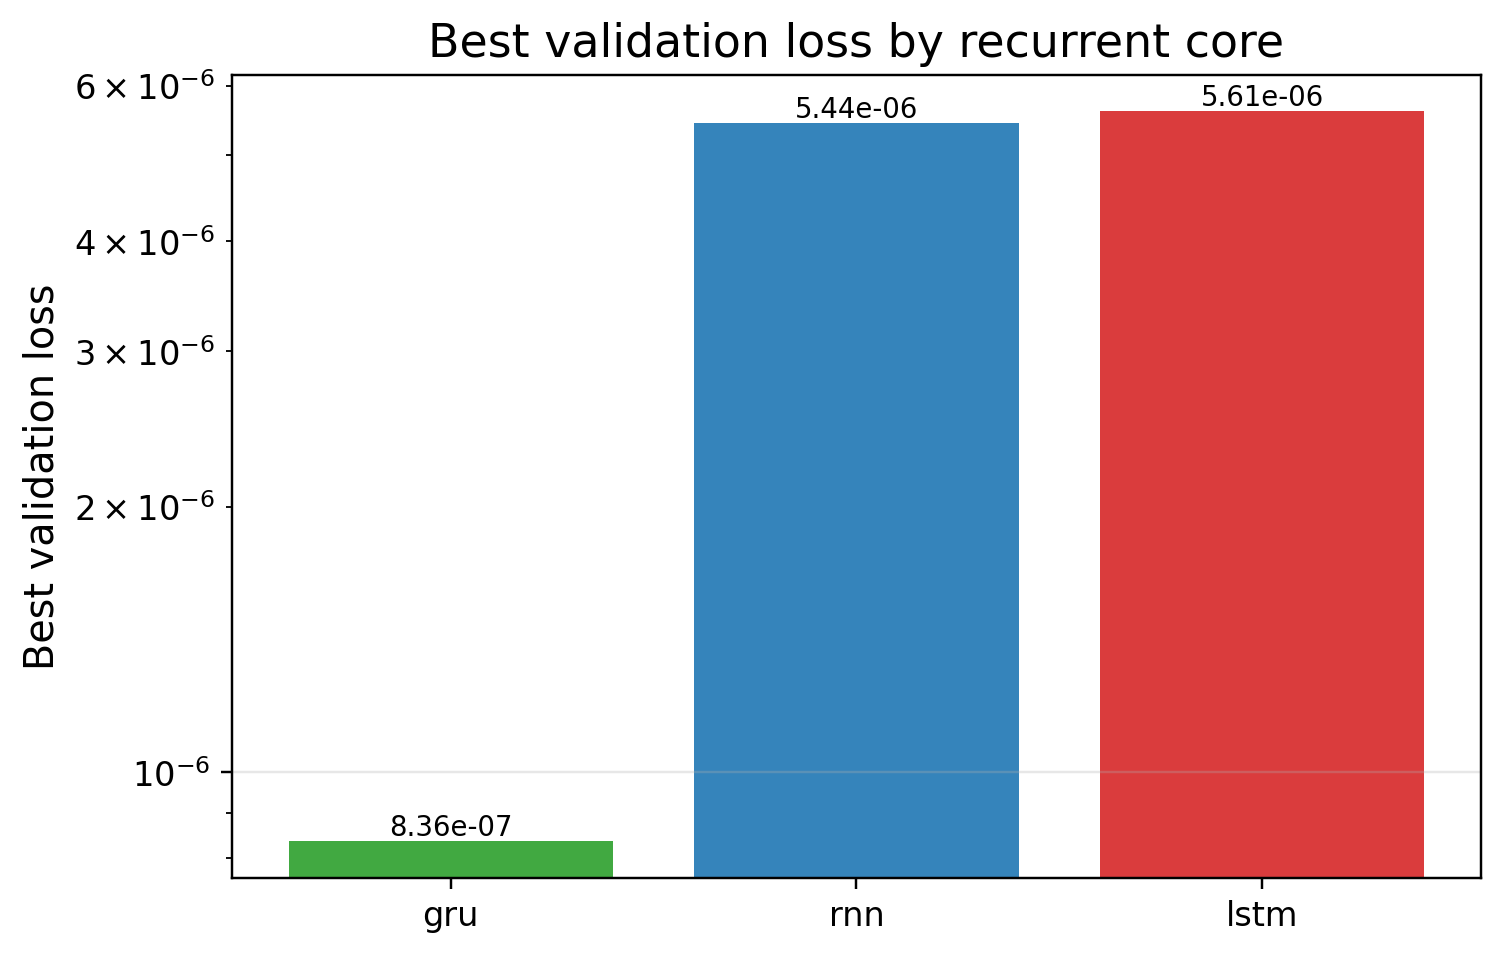
\includegraphics[width=\textwidth]{optuna/02_family_best_validation_loss.png}
    \caption{Best validation loss by cell family.}
\end{subfigure}
\hfill
\begin{subfigure}[h]{0.49\textwidth}
    \centering
    
\includegraphics[width=\textwidth]{figures/optuna/02_family_best_trial_runtime.png}
    \caption{Runtime of best trial by cell family.}
\end{subfigure}
\hfill
\begin{subfigure}[h]{0.95\textwidth}
    \centering
    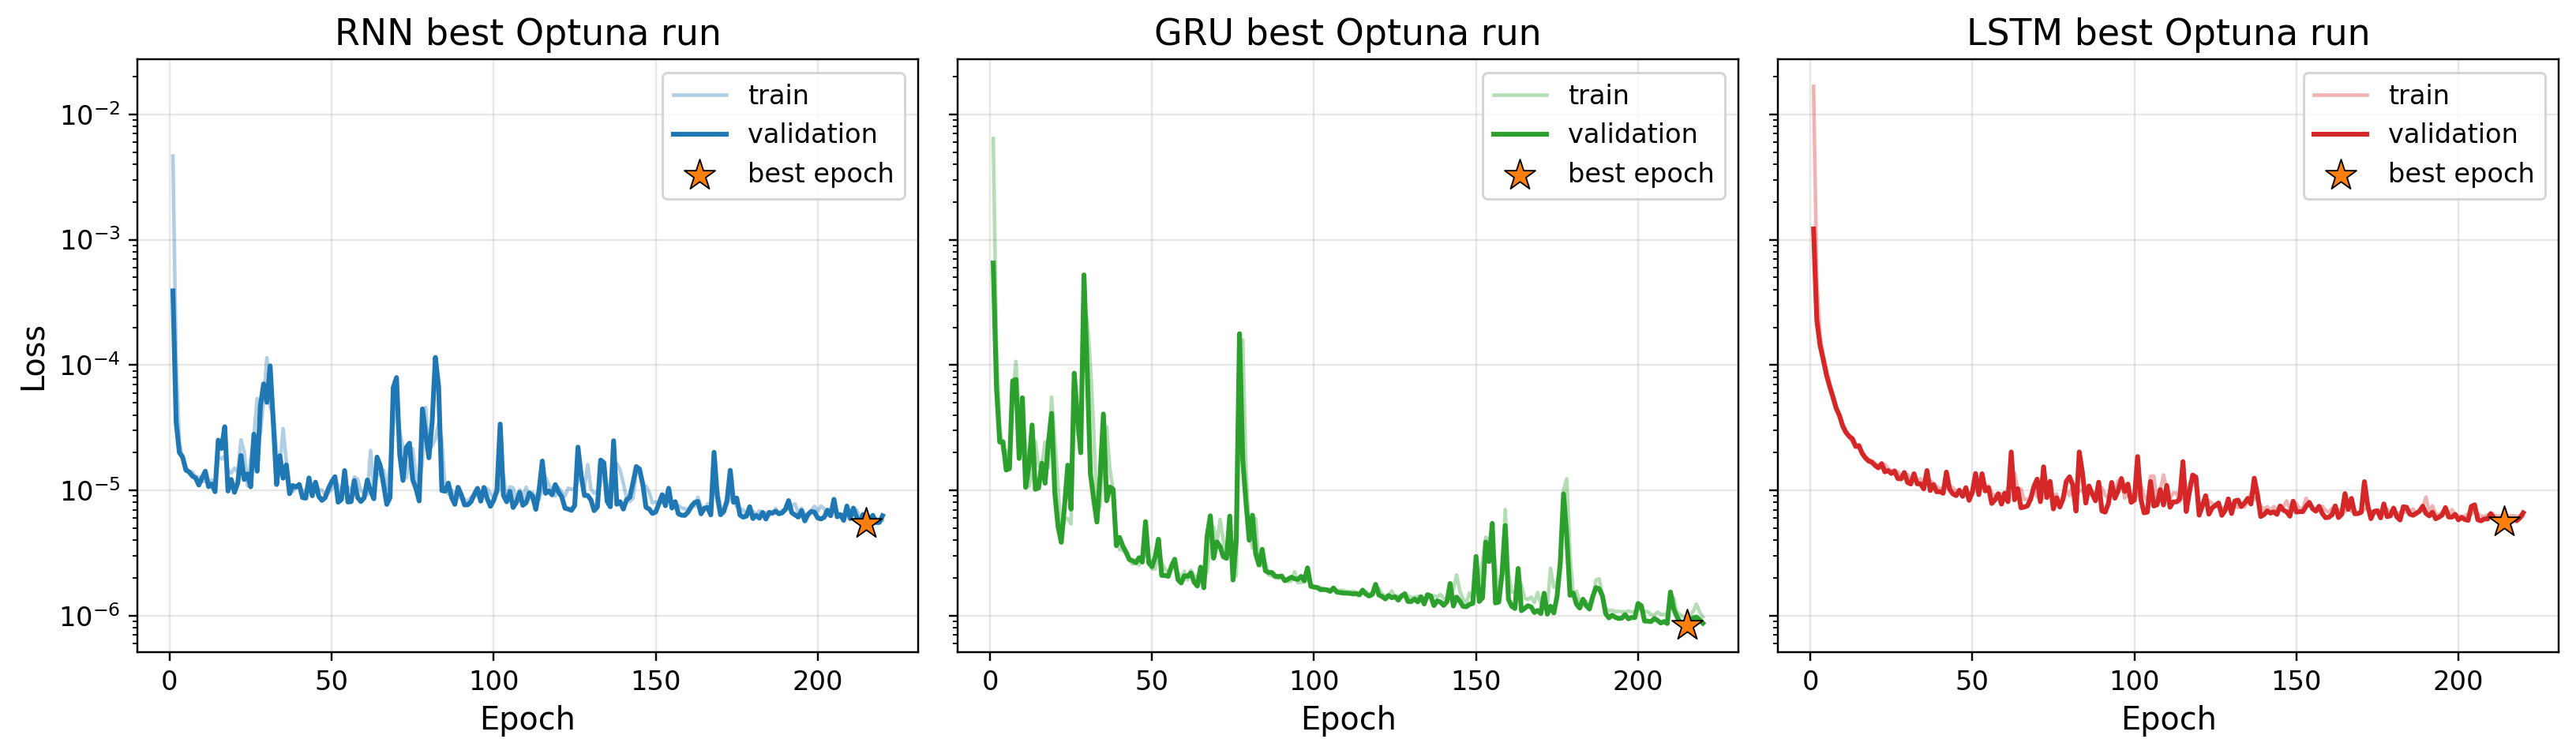
\includegraphics[width=\textwidth]{optuna/02_best_optuna_training_curves.png}
    \caption{Training and validation curves for the best trial in each family (light colour being train loss).}
\end{subfigure}
\caption{Optuna architecture search over vanilla RNN, GRU, and LSTM. GRU achieved the lowest validation loss by a clear margin, while LSTM plateaued earlier and at a higher loss despite having the most flexible gating mechanism.}
\label{fig:optuna_search_summary}
\end{figure}

\begin{figure}[h]
\centering
\begin{subfigure}[h]{0.47\textwidth}
    \centering
    
\includegraphics[width=\textwidth]{optuna/02_gru_param_importance.png}
    \caption{Optuna parameter importance for the GRU study.}
\end{subfigure}
\hfill
\begin{subfigure}[h]{0.47\textwidth}
    \centering
    
\includegraphics[width=\textwidth]{optuna/02_gru_loss_vs_hidden.png}
    \caption{GRU validation loss against hidden dimension across the Optuna trials.}
\end{subfigure}
\caption{Optimisation details for the winning GRU family. The hidden dimension is the dominant optimisation variable, while the trial scatter also shows that hidden-size effects are not perfectly sharp even before the more focused threshold studies.}
\label{fig:gru_optuna_detail}
\end{figure}

Whilst Figure~\ref{fig:gru_optuna_detail} shows that higher hidden dimensions and low batch sizes are generally better, it should be noted that the range of losses on the absolute scale is small across all 3 families of models. Whilst the hyperparameter tuning showed very good performance, with a best validation loss as low as $8.36 \times 10^{-7}$, it seems in hindsight that this was not needed, particularly with 90 trials explored with long run times. For this reason, further experiments with the forward Euler-based models were done with no hyperparameter tuning and a time-optimised batch size of 32. This focus shift reflects the models themselves, shifting from a focus on performance with the cell-based RNOs to a focus on physical insight with the Euler-based RNOs.

\FloatBarrier
\section{Cell-based Architecture Performance Results}

\subsection{Best Predictive Model From The Architecture Search}

Table~\ref{tab:cell_model_comparison} summarises the best predictive model from each family together. The GRU achieved the lowest validation loss and the lowest test errors overall. Its test relative $L^2$ error was $3.72\times 10^{-3}$ and its coefficient of determination was $0.999986$, making it the strongest predictive model in the study, however all three models were very strong.


\begin{table}[h]
\centering
\caption{Best independently tuned cell-based models.}
\label{tab:cell_model_comparison}
\begin{tabular}{lcccc}
\toprule
Model & Best val. loss & Test RMSE & Test relative $L^2$ & Test $R^2$ \\
\midrule
GRU & $8.36\times 10^{-7}$ & $1.26\times 10^{-3}$ & $3.72\times 10^{-3}$ & $0.999986$ \\
RNN & $5.44\times 10^{-6}$ & $3.02\times 10^{-3}$ & $8.91\times 10^{-3}$ & $0.999920$ \\
LSTM & $5.61\times 10^{-6}$ & $3.09\times 10^{-3}$ & $9.12\times 10^{-3}$ & $0.999916$ \\
\bottomrule
\end{tabular}
\end{table}


The performance of the GRU is consistent with the training curves in Figure~\ref{fig:optuna_search_summary}. The LSTM did not outperform the GRU, even though it has the most expressive gating mechanism. The most plausible explanation is that the dataset is not large enough to reward the extra flexibility of a full cell-state architecture. The LSTM may also be suited to materials with slower rate behaviour, as discussed earlier about the validation losses. The GRU appears to provide the best trade-off between memory capacity and optimisation difficulty. In contrast, the vanilla RNN is most exposed to gradient degradation over long sequences, and the LSTM pays a higher parameter and optimisation cost without a corresponding generalisation gain.

The baseline RNO sits between the GRU and the other cell-based models. This is an important result: a custom state-space constitutive operator can be competitive, but in this dataset, the best purely predictive model is still the gated GRU. 

A small note on the computation backend: All final reported results were run on CPU. Although Apple MPS was available, the explicit time-sequence loop made CPU execution faster in practice for this workload. This was tested reasonably thoroughly, but the results were deemed outside of the importance or scope of the coursework brief.

\subsection{Qualitative Behaviour Of The Best GRU Model}

The best GRU was evaluated on the held-out test set and on unseen cyclic loading. Figure~\ref{fig:qualitative_test_examples} shows the best, median, and worst test trajectories in both stress-time and stress-strain space. Even the worst selected example remains physically plausible and follows the correct loop orientation. The largest deviations occur around turning points and steep changes in slope, with small ``overshoots'' being observed, however these are very small and somewhat indistinguishable in Figure~\ref{fig:qualitative_test_examples}. This is consistent with a recurrent model that has learned the broad constitutive structure but still accumulates its largest errors where history and rate interact most strongly. This could be explained somewhat by the 1-step update lag for strain rate, hence the immediate correction after these small overshoots that continue based on the trajectory of the last step.

\begin{figure}[h]
\centering
\begin{subfigure}[h]{0.8\textwidth}
    \centering
    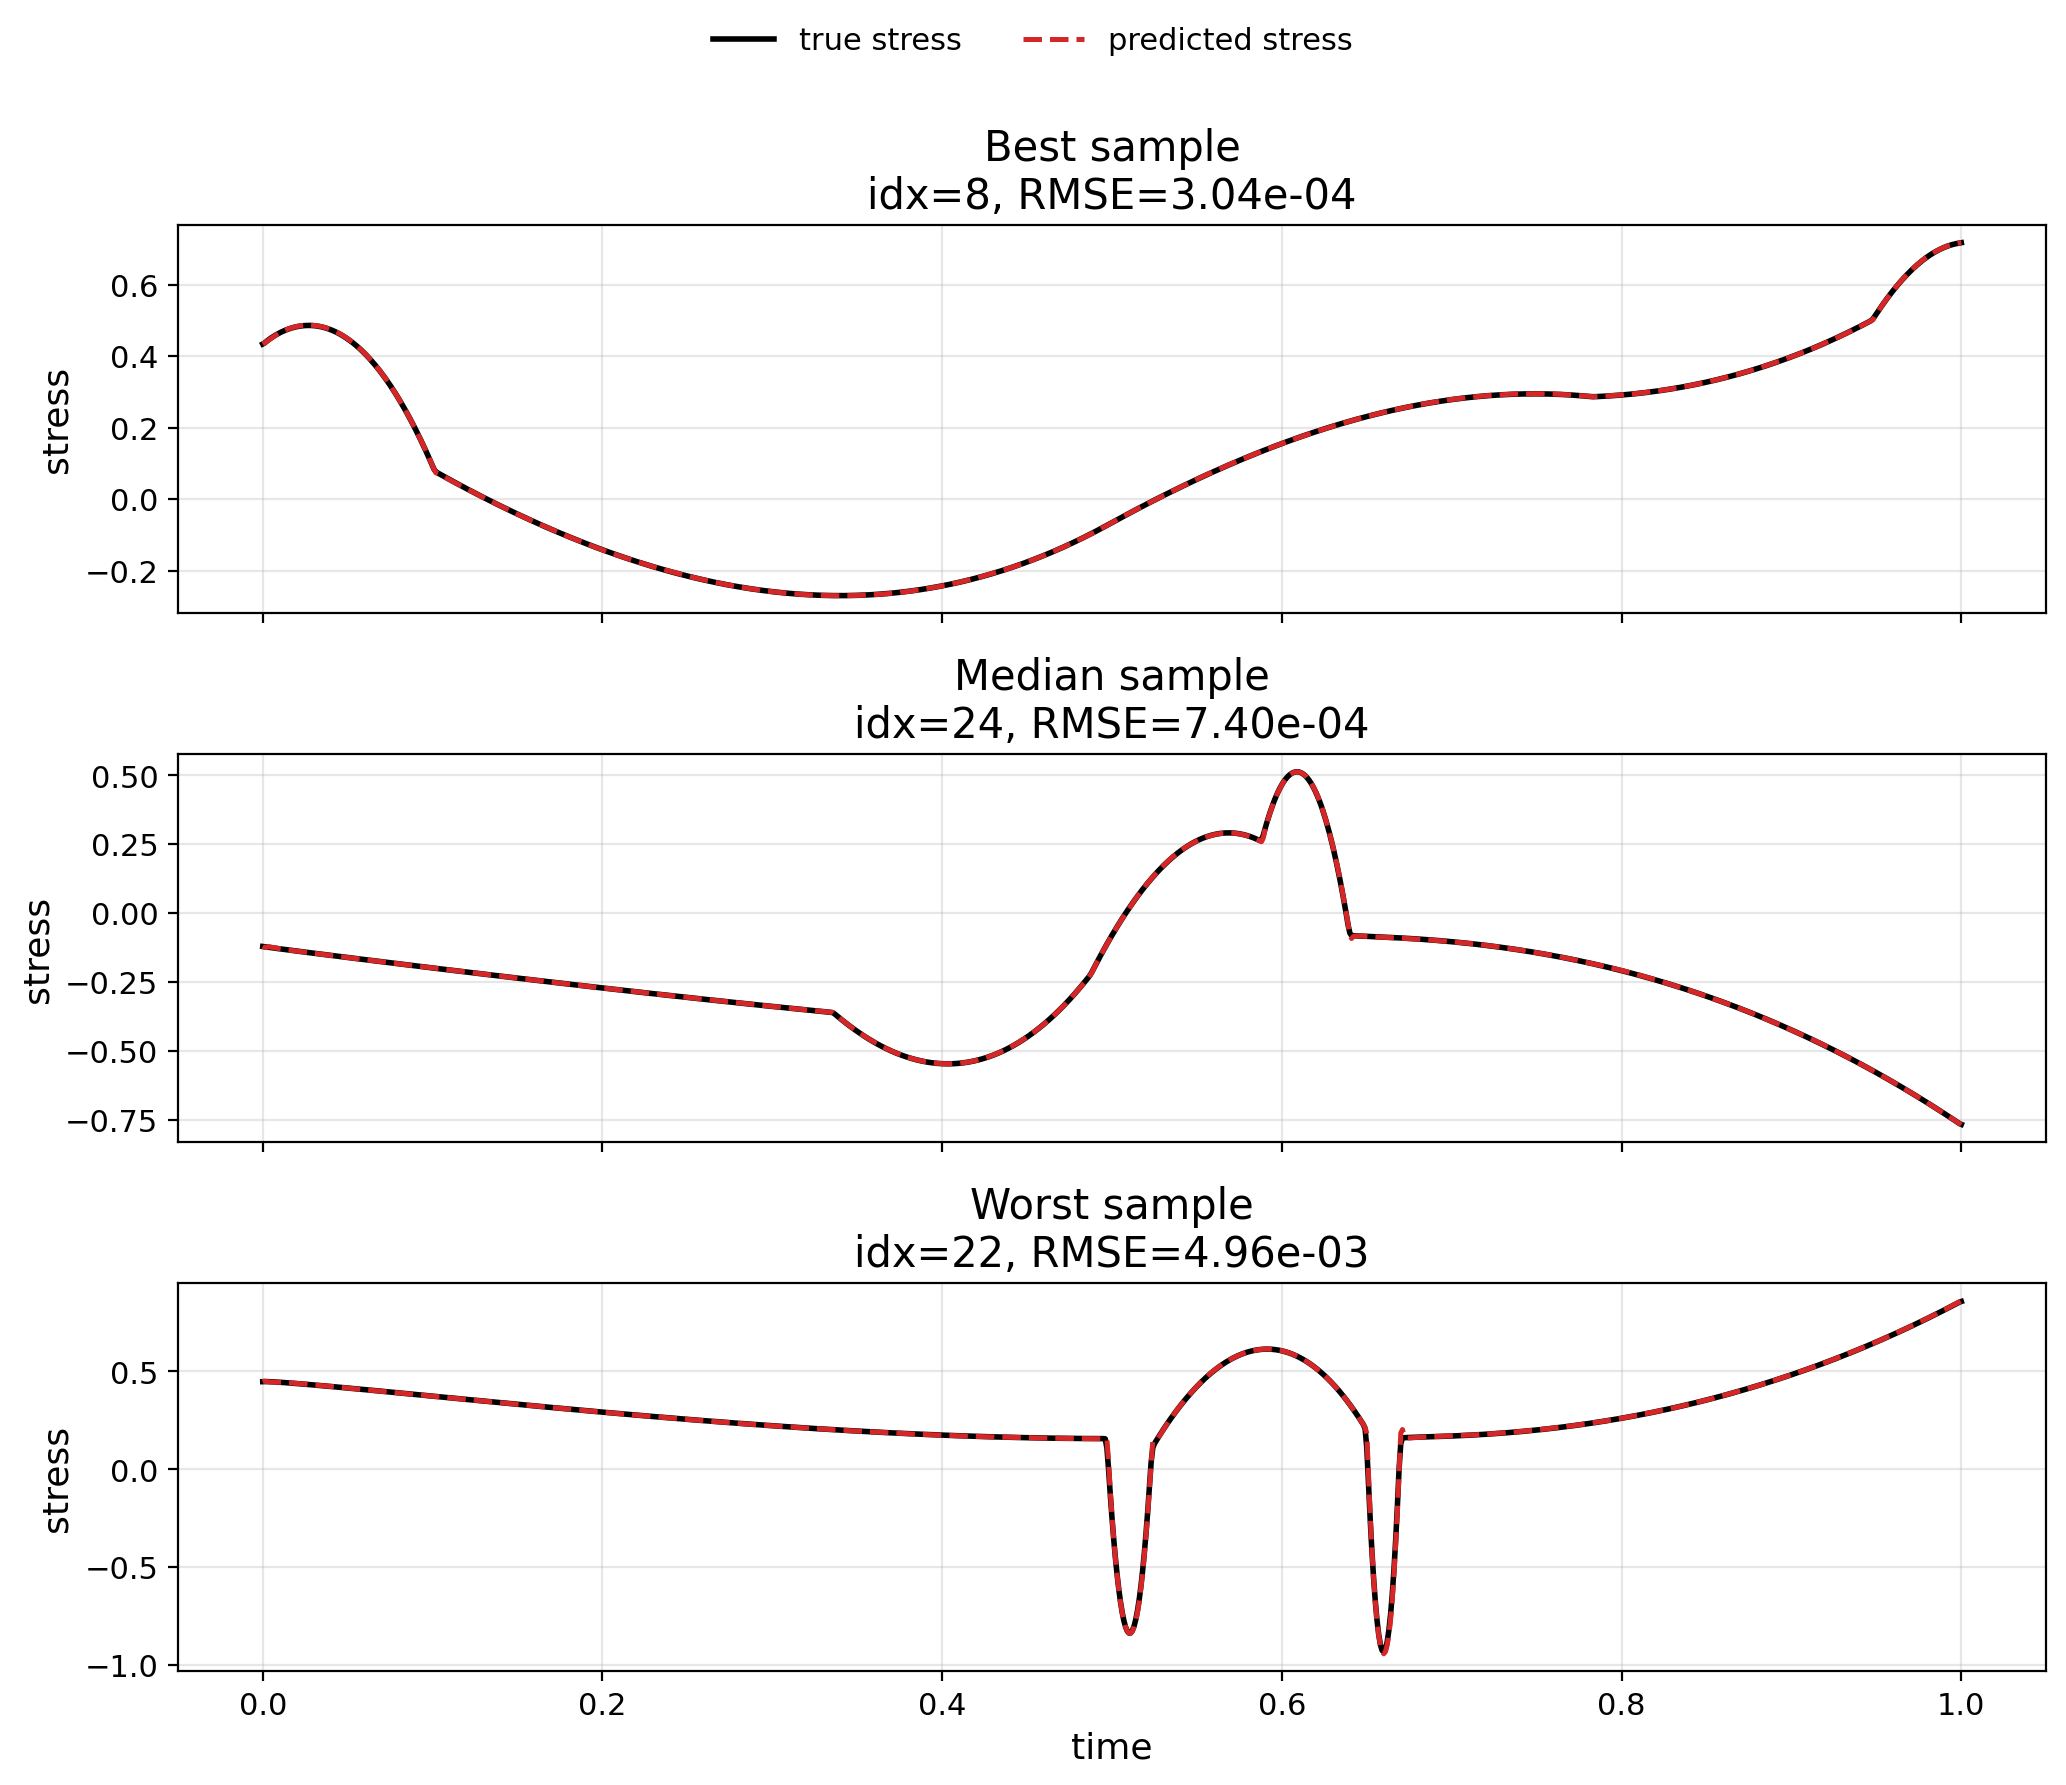
\includegraphics[width=\textwidth]{05_test_stress_time_examples.png}
    \caption{Stress histories in time for best, median, and worst test samples.}
\end{subfigure}
\begin{subfigure}[h]{0.95\textwidth}
    \centering
    
\includegraphics[width=\textwidth]{05_test_stress_strain_examples.png}
    \caption{Stress--strain trajectories for the same three test samples.}
\end{subfigure}
\caption{Qualitative behaviour of the best Optuna GRU on the test set. The model captures the overall constitutive loops very well, while the remaining errors concentrate near sharp turning points and the highest-curvature portions of the trajectories.}
\label{fig:qualitative_test_examples}
\end{figure}

\FloatBarrier

Figure~\ref{fig:hysteresis_and_residuals} complements these trajectory plots. The residual plot shows that the best GRU has small, mostly structureless errors on the test set, while the unseen cyclic tests show that the model reproduces hysteresis loops rather than collapsing to an elastic single-valued response. This matters because a visually good time-series fit alone would not prove that the model has learned a meaningful constitutive relation. We can also see the small overshoots in the sharper hysteresis check plot.

\begin{figure}[h]
\centering
\begin{subfigure}[h]{0.7\textwidth}
    \centering
    
\includegraphics[width=\textwidth]{04_residual_analysis_top_row.png}
    \caption{Residual analysis for the best GRU on the held-out test set.}
\end{subfigure}
\hfill
\begin{subfigure}[h]{0.8\textwidth}
    \centering
    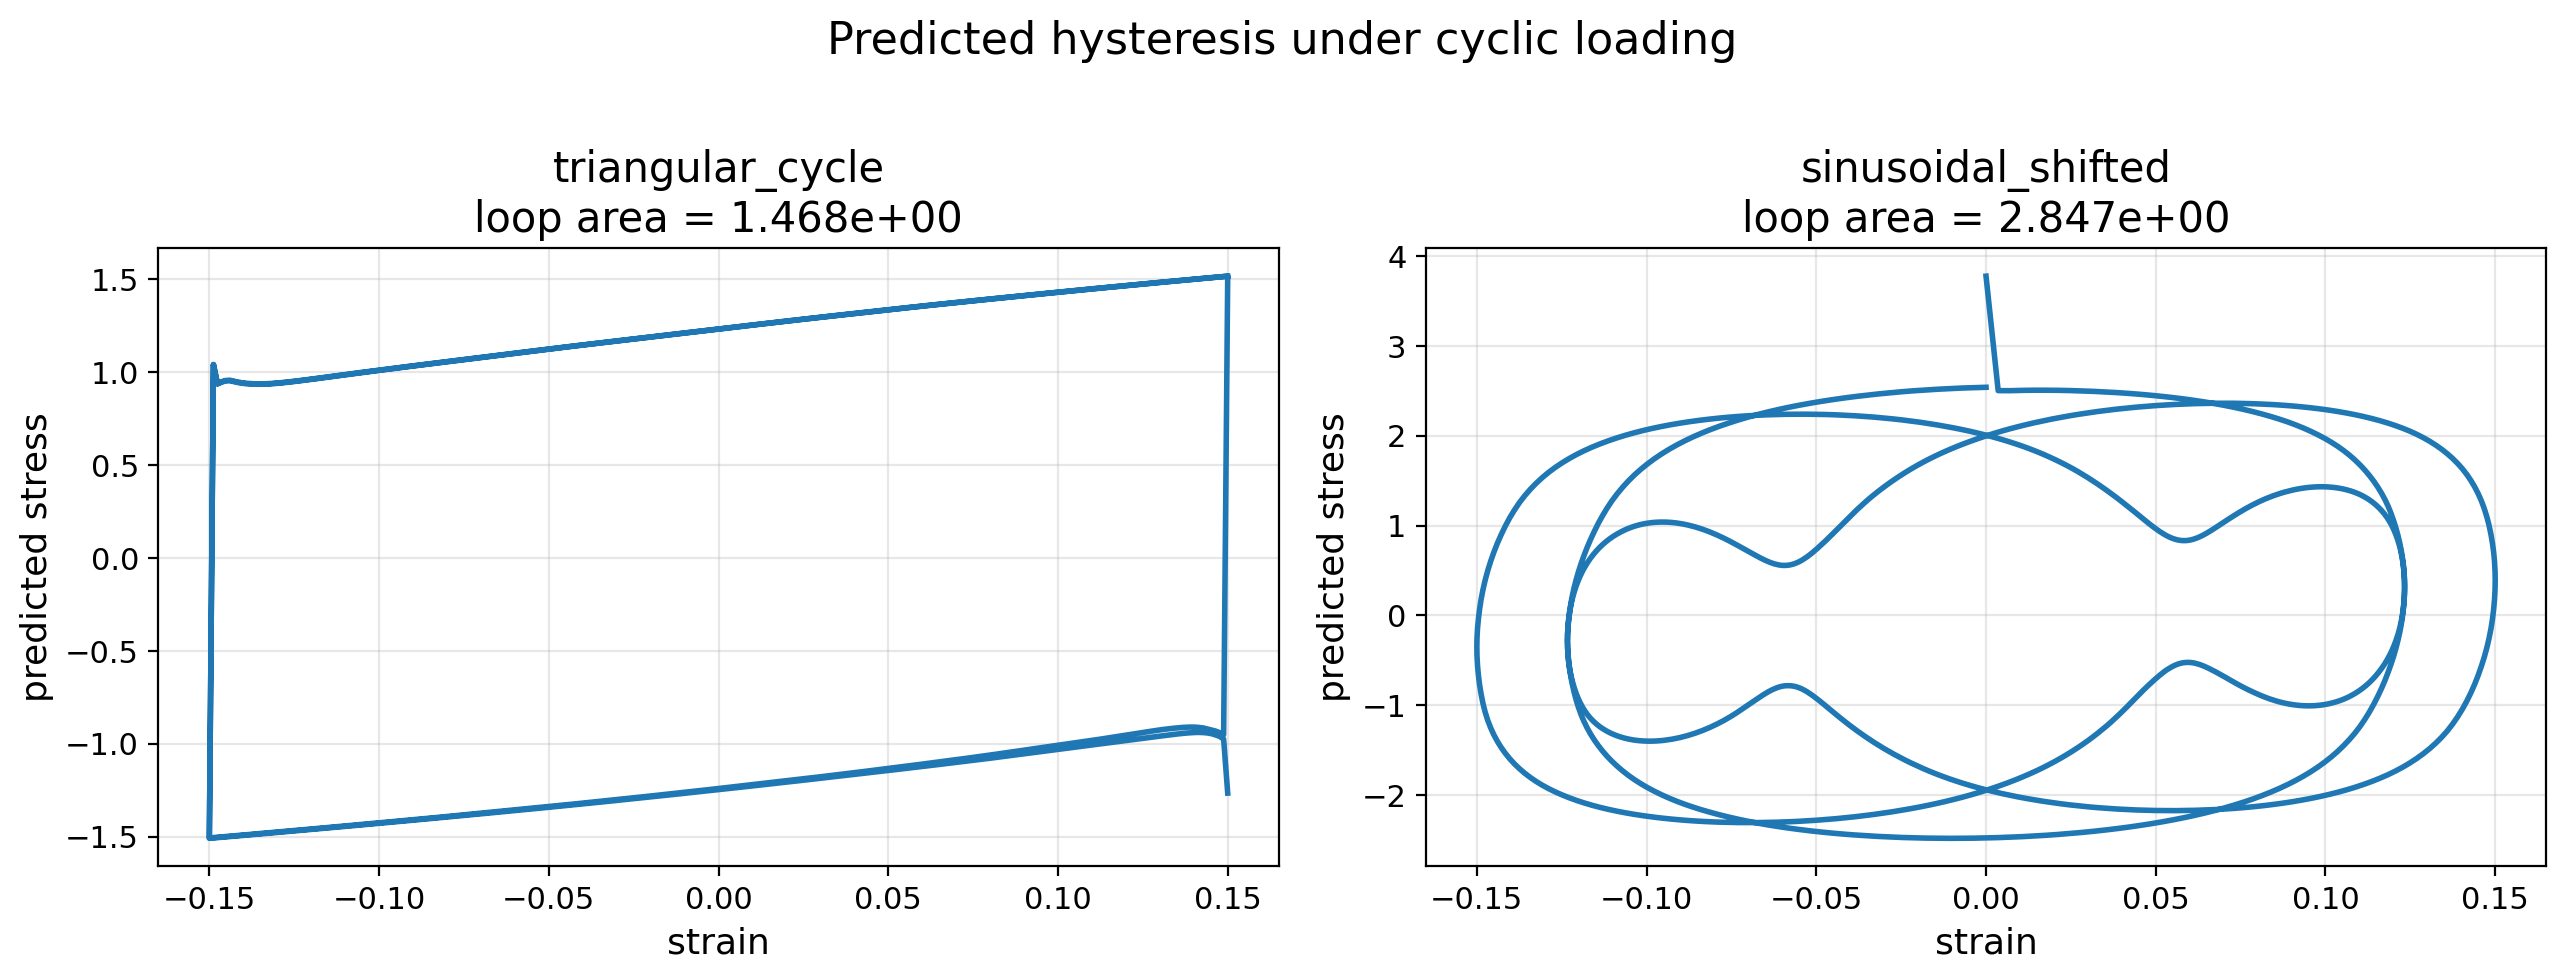
\includegraphics[width=\textwidth]{05_hysteresis_checks.png}
    \caption{Predicted hysteresis under unseen cyclic loading.}
\end{subfigure}
\caption{Additional qualitative checks for the best GRU. The residuals are small and unbiased overall, while the unseen cyclic tests demonstrate that the model reproduces looped, rate-dependent behaviour rather than a purely elastic stress--strain curve.}
\label{fig:hysteresis_and_residuals}
\end{figure}

\subsection{Unseen Load Predictions}
\label{sec:unseen_predictions}

To test whether the best GRU had learned a constitutive operator rather than only reproducing trajectories drawn from the train/validation/test split, the model was also evaluated on four hand-crafted loading paths that were not taken directly from the dataset: a monotonic ramp, a ramp--hold loading path, a triangular cycle, and a shifted multi-frequency sinusoidal loading path. The resulting predictions are shown in Figure~\ref{fig:unseen_predictions}. Since no reference stress solution was generated for these trajectories, this part of the analysis is qualitative rather than error-based. The aim was to assess whether the predicted responses remain physically plausible under loading histories with different temporal structures.

\begin{figure}[h]
    \centering
    
\includegraphics[width=0.8\textwidth]{04_unseen_predictions.png}
    \caption{Unseen loading paths and the corresponding free-running stress predictions from the best GRU model. The left column shows the imposed strain histories and the right column shows the predicted stress response for each case.}
    \label{fig:unseen_predictions}
\end{figure}

Several concise observations can be made from Figure~\ref{fig:unseen_predictions}. The monotonic ramp produces a smooth and bounded increase in stress, indicating that the model remains stable under a simple unseen loading programme. The ramp-hold case is more revealing: the stress reaches a peak at the end of the ramp, then drops sharply when the strain rate switches to zero, before settling toward a lower positive plateau. This suggests that the GRU has learned a strong rate-dependent contribution, but that abrupt changes in loading rate are not captured perfectly smoothly. This suggests the viscoelastic behaviour of the model has an extremely quick decay time, almost reminiscent of frictional forces.

The two reversing cases provide clearer evidence of constitutive memory. In both the triangular-cycle and shifted-sinusoidal inputs, the predicted stress remains bounded and responds systematically to repeated reversals, rather than collapsing to a single-valued instantaneous stress-strain response. The triangular case shows that these reversals are handled with abrupt sign changes rather than smooth transitions, which is consistent with the model being strongly sensitive to discrete changes in loading direction.

The shifted-sinusoidal case provides clear evidence of constitutive memory as well, combining multiple frequencies in the strain. Although the strain repeatedly changes sign, the stress response remains smooth and bounded, and does not reverse sign instantaneously at the same points, indicating a phase-lagged, history-dependent response rather than a single-valued instantaneous stress-strain relation.

One important caveat is that these unseen predictions are free-running: unlike the standard train/validation/test evaluations, the first stress value is estimated using the fitted initial-rate model rather than pinned to a known target. Consequently, the most meaningful part of Figure~\ref{fig:unseen_predictions} is the subsequent constitutive evolution, especially the stable monotonic response, the sharp rate-switch correction in the ramp-hold case, and the path-dependent sign changes under cyclic loading.


\section{Initial Hidden Parameter Analysis}

Experiments were conducted to determine the minimum number of internal/hidden variables required in the RNO to fully learn the
constitutive relation, as per part (c). Note this section was the initial analysis for this, and the motivation for the next section, which explores a different family of models with different architectures from the cell-based method.

\FloatBarrier
\subsection{Operational Definition Of ``Fully Learned''}

Part (c) asks for the minimum number of hidden or internal variables required to ``fully learn'' the constitutive relation. That phrase is not mathematically unique, so an operational criterion was needed. As a starting point, throughout the hidden-size studies, the minimum acceptable hidden dimension was defined as the smallest $h$ whose validation loss lay within $5\%$ of the best validation loss in the relevant sweep or reference study. \textbf{This was used purely as a guide} whilst running the experiments. Formally, if the best validation loss in the comparison set is $L_{\min}$, then the acceptance threshold is
\begin{equation}
L_{\mathrm{th}}=1.05\,L_{\min}.
\label{eq:threshold_definition}
\end{equation}
The selected hidden size is then
\begin{equation}
h_{\mathrm{sel}}=\min\left\{h: L(h)\leq L_{\mathrm{th}}\right\}.
\label{eq:hidden_selection_rule}
\end{equation}
This criterion does not claim to identify a unique physical truth. Instead, it provides a reproducible rule for distinguishing ``smallest hidden size that is effectively as good as the best tested model'' from ``smallest hidden size that merely gives a plausible curve''. That distinction becomes important once the hidden-size curves turn out to be smooth rather than cliff-like.

It should be noted that this was initially implemented as a starting point, and as we shall see, due to the relative nature of this criterion, it is a \textbf{within-model} criterion, rather than a global criterion. This makes it a reasonably weak criterion, but we shall use it as a guide nonetheless to try to provide some insight into the models. 

The definition of the fully learned criterion was difficult due to results showing somewhat unexpected behavior, as we will discuss.



\FloatBarrier
\subsection{Initial Hidden-Size Sweep On The Best GRU}

The first attempt to answer part (c) was to freeze the best non-hidden hyperparameters from the winning GRU and sweep the hidden size downward. The result is shown in Figure~\ref{fig:gru_threshold_attempt}. The key observation is that the error improves smoothly from $h=0$ to $h=4$ rather than exhibiting a dramatic cliff. The mean validation loss decreases from $8.38\times 10^{-6}$ at $h=0$ to $3.27\times 10^{-6}$ at $h=4$, but no value in the tested range reached the strict $5\%$ threshold relative to the Optuna-best GRU.

\begin{figure}[h]
\centering

\includegraphics[width=0.78\textwidth]{hidden_threshold_low_dim_with_reference_threshold.png}
\caption{Low-dimensional hidden-size sweep for the best GRU recipe, compared with the cached $h=4$ reference. The trend is monotonic but smooth, and no hidden size in $\{0,1,2,3,4\}$ met the strict $5\%$ threshold defined relative to the Optuna-best GRU result.}
\label{fig:gru_threshold_attempt}
\end{figure}

This apparently inconclusive result is already informative. In the GRU formulation, the model is given the explicit feature vector from Equation~\eqref{eq:step_features}, so the $h=0$ case is \emph{not} a truly memoryless constitutive law. Even without latent state, it still receives the current strain, previous strain, and discrete strain rate directly. That makes the zero-hidden case much stronger than the clean internal-variable test considered by Liu et al.~\cite{Liu_2023}, and it explains why the threshold is not sharply defined. With a loss of $8.38\times 10^{-6}$ at $h=0$, it could be argued that the hidden variables are not needed for the model to fully learn the constitutive relationship. This is also why the 5\% threshold was used as a guide only, as the absolute loss is arguably more important.

This was not a satisfactory result, and so alternate architectures were explored in order to attempt to answer this part of the coursework more thoroughly.




\FloatBarrier

\section{Follow-Up Method: Explicit Forward Euler Recurrent Models}

\subsection{Architecture}

A second method family was introduced because the initial hidden-dimension study with the best GRU model did not reveal a clear or physically interpretable minimum hidden-state threshold, with the hypothesis that a more explicit state-space formulation was needed for part~(c). The hope with this family of models was to achieve a more defined threshold of a minimum number of hidden variables.

This second model family follows the internal-variable viewpoint of Liu et al.~\cite{Liu_2023}, as well as the skeleton code provided in the coursework brief, to study hidden variables in a more explicitly state-space form. Two variants were used, both retaining the similar feature-lifting and stress-readout MLPs as in the cell-based models. This preserves the outer recurrent constitutive-operator structure and allows the comparison to focus specifically on the different hidden-state evolution laws described below. The exception to this is a change to the stress-readout as discussed below.


\paragraph{Baseline RNO.}
The first variant stays close to the coursework skeleton. Its hidden state evolves by an explicit Euler step,
\begin{equation}
\bm{h}_n=\bm{h}_{n-1}+\dt\,\bm{g}\!\left(\epsbar_{n-1},\bm{h}_{n-1}\right),
\label{eq:baseline_state_update}
\end{equation}
and the stress is read out from previous strain, discrete strain rate, and the hidden state,
\begin{equation}
\hat{\sigbar}_n=f\!\left(\epsbar_{n-1},\frac{\epsbar_{n-1}-\epsbar_n}{\dt},\bm{h}_{n-1}\right).
\label{eq:baseline_readout}
\end{equation}
This model was used because it is much closer to the supplied RNO skeleton than the standard cell-based architectures.

\paragraph{Paper-inspired RNO.}
The second variant follows the cleaner state-space form proposed by Liu et al.~\cite{Liu_2023}. In its most general form,
\begin{equation}
\hat{\sigbar}_n=f\!\left(\epsbar_n,\dot{\epsbar}_n,\bm{h}_{n}\right),
\label{eq:paper_stress_relation}
\end{equation}
\begin{equation}
\bm{h}_{n}=\bm{h}_{n-1}+\dt\,\bm{g}\!\left(\epsbar_n,\bm{h}_{n-1}\right).
\label{eq:paper_kinetic_relation}
\end{equation}
Two cases were tested:
\begin{enumerate}[leftmargin=1.5em]
    \item \textbf{No-rate paper RNO:} the stress readout uses only $\epsbar_n$ and $\bm{h}_n$,
    \item \textbf{With-rate paper RNO:} the stress readout uses $\epsbar_n$, $\dot{\epsbar}_n$, and $\bm{h}_n$.
\end{enumerate}
The distinction is critical. In the no-rate model, the hidden state is forced to carry essentially all of the constitutive memory. In the with-rate model, part of the relevant physics is supplied explicitly through the strain-rate channel.

This separation is also relevant to the hidden-size question. If $h=0$ in the no-rate paper RNO, the constitutive law collapses to an instantaneous map
\begin{equation}
\hat{\sigbar}_n=f\!\left(\epsbar_n\right),
\label{eq:h0_no_rate}
\end{equation}
which is structurally incapable of representing a general history-dependent constitutive law. If $h=0$ in the with-rate model, the constitutive law becomes
\begin{equation}
\hat{\sigbar}_n=f\!\left(\epsbar_n,\dot{\epsbar}_n\right),
\label{eq:h0_with_rate}
\end{equation}
which is still memoryless in the latent sense, but is much stronger because the rate effect is supplied directly.

This family of models was introduced specifically to obtain a more well-defined and physically interpretable answer to part~(c). The baseline RNO was included as the simplest model that remained close to the provided skeleton code, while the paper-inspired RNO variants were used to test whether the sharper loss transitions and hidden-variable thresholds reported by Liu et al.~\cite{Liu_2023} would also emerge for the viscoelastic composite dataset being tested. 

As mentioned earlier, experiments with the forward Euler-based models were done with no hyperparameter tuning and a time-optimised batch size of 32. This was done in order to efficiently explore the hidden parameter threshold behaviour. It is for this reason that these models cannot be compared to the previous highly tuned models, as it is an unfair comparison.


\subsection{Follow-Up Method Hidden Parameter Analysis}
\label{sec:operator_hidden_dimension}

Because the GRU hidden sweep did not reveal a sharp or easily interpretable minimum hidden dimension, the analysis was extended to the three more explicitly state-space models discussed above: the baseline RNO, and two paper-inspired RNO variants with and without explicit strain-rate input in the stress readout. To make a broader hidden-dimension sweep feasible, all three operator-style studies in this section were run on CPU with batch size $32$ with an accelerated stopping protocol. The effect of batch size on accuracy was explored and shown to be negligible in the context of defining the minimum hidden parameters. The resulting curves are shown in Figure~\ref{fig:operator_hidden_sweeps}, and the corresponding validation losses are summarised in Tables~\ref{tab:operator_hidden_losses} and~\ref{tab:operator_threshold_summary}.

\begin{figure}[h]
\centering
\begin{subfigure}[h]{0.6\textwidth}
    \centering
    
\includegraphics[width=\textwidth]{figures/07_baseline_rno_batch32_accel_hidden_grid_0to4_threshold.png}
    \caption{Baseline RNO.}
    \label{fig:baseline_hidden_sweep}
\end{subfigure}
\hfill
\begin{subfigure}[h]{0.48\textwidth}
    \centering
    
\includegraphics[width=\textwidth]{09_paper_rno_no_rate_h0to5_threshold.png}
    \caption{No-rate paper RNO threshold view.}
\end{subfigure}
\hfill
\begin{subfigure}[h]{0.48\textwidth}
    \centering
    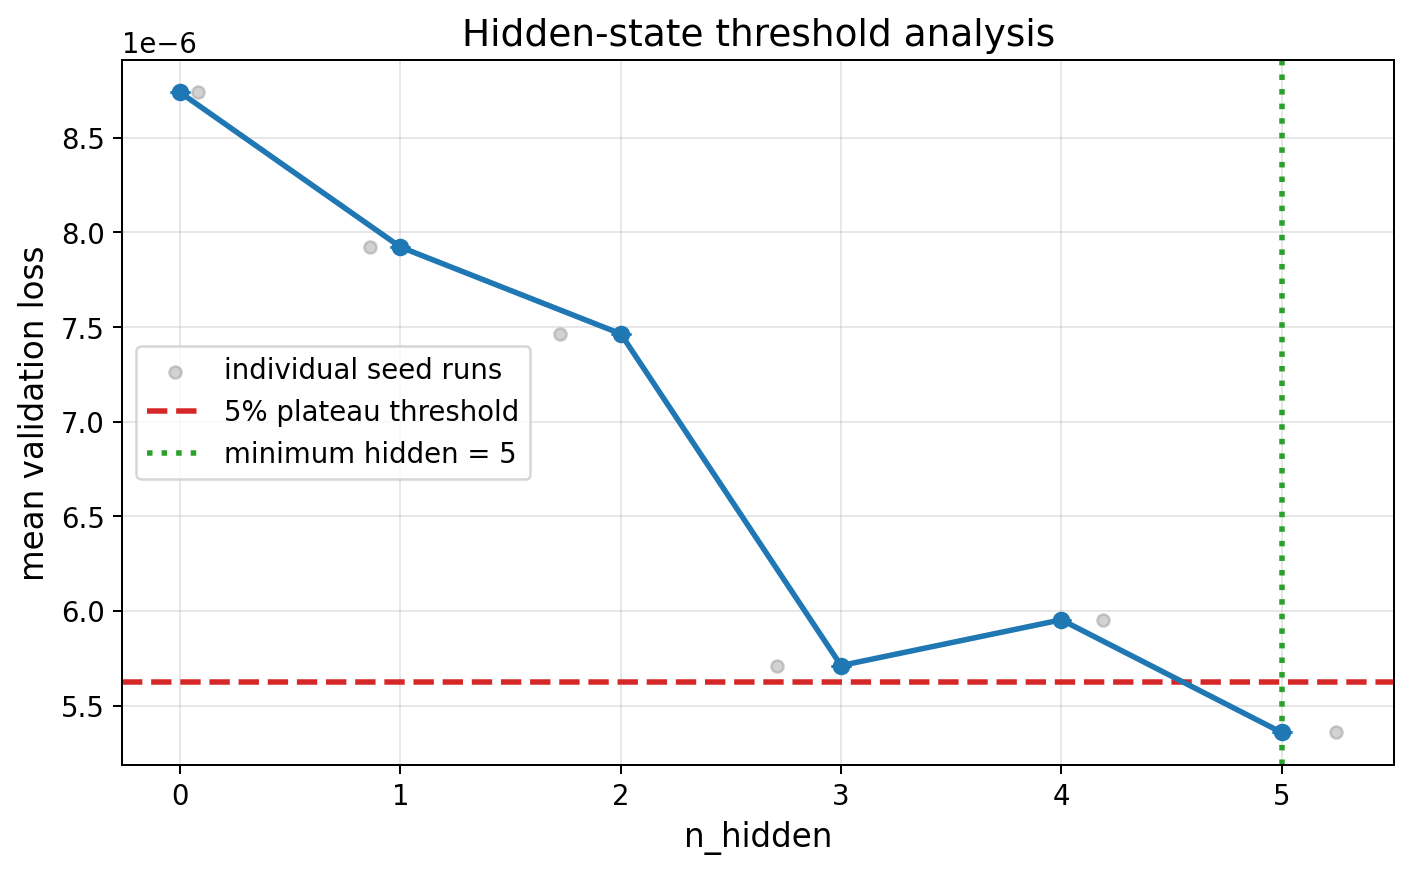
\includegraphics[width=\textwidth]{09_paper_rno_with_rate_h0to5_threshold.png}
    \caption{With-rate paper RNO threshold view.}
\end{subfigure}
\caption{Hidden-dimension sweeps for the operator-style models, all evaluated with batch size $32$. The baseline RNO was swept over $h=0,\dots,4$, while the two paper-inspired variants were swept over $h=0,\dots,5$.}
\label{fig:operator_hidden_sweeps}
\end{figure}


\begin{table}[h]
\centering
\caption{Mean validation loss against hidden dimension for the operator-style sweeps. All runs used batch size $32$.}
\label{tab:operator_hidden_losses}
\begin{tabular}{lcccccc}
\toprule
Model & $h=0$ & $h=1$ & $h=2$ & $h=3$ & $h=4$ & $h=5$ \\
\midrule
Baseline RNO
& $8.75\times10^{-6}$
& $7.27\times10^{-6}$
& $7.18\times10^{-6}$
& $8.20\times10^{-6}$
& $5.82\times10^{-6}$
& -- \\
Paper RNO, no rate
& $3.98\times10^{-2}$
& $3.52\times10^{-2}$
& $2.36\times10^{-2}$
& $1.91\times10^{-2}$
& $1.86\times10^{-2}$
& $1.92\times10^{-2}$ \\
Paper RNO, with rate
& $8.74\times10^{-6}$
& $7.92\times10^{-6}$
& $7.46\times10^{-6}$
& $5.71\times10^{-6}$
& $5.95\times10^{-6}$
& $5.36\times10^{-6}$ \\
\bottomrule
\end{tabular}
\end{table}

\begin{table}[h]
\centering
\caption{Threshold-style summary for the operator-style hidden-dimension sweeps, using the smallest hidden dimension within $5\%$ of the best validation loss found in each sweep.}
\label{tab:operator_threshold_summary}
\begin{tabular}{lccccc}
\toprule
Model & Hidden grid & Best tested $h$ & Best val. loss & $5\%$ limit & Selected $h$ \\
\midrule
Baseline RNO
& $0,1,2,3,4$
& $4$
& $5.82\times10^{-6}$
& $6.11\times10^{-6}$
& $4$ \\
Paper RNO, no rate
& $0,1,2,3,4,5$
& $4$
& $1.86\times10^{-2}$
& $1.95\times10^{-2}$
& $3$ \\
Paper RNO, with rate
& $0,1,2,3,4,5$
& $5$
& $5.36\times10^{-6}$
& $5.63\times10^{-6}$
& $5$ \\
\bottomrule
\end{tabular}
\end{table}

\FloatBarrier

Several distinct behaviours emerge from Figure~\ref{fig:operator_hidden_sweeps} and Table~\ref{tab:operator_hidden_losses}. The baseline RNO improves modestly as the hidden dimension increases, but the curve is not cleanly monotone, and the best result occurs at the edge of the tested range, $h=4$. Under the $5\%$ rule in Table~\ref{tab:operator_threshold_summary}, this selects $h=4$, but this should be interpreted cautiously: it is better described as a best-tested value than as a clear physical threshold, particularly as it is relative to the best case within the model, guaranteeing at least one successful trial that reaches the threshold, as that trial will define the threshold. Relative to the best GRU, the baseline RNO remains less accurate, but it is still useful as the closest operator-style comparator to the original skeleton code.

The paper-inspired no-rate RNO gives the clearest threshold-like behaviour. Its loss drops substantially from $h=0$ to $h=3$, then changes only weakly between $h=3$, $h=4$, and $h=5$. This is the cleanest threshold result for part~(c), and the $5\%$ rule therefore selects $h=3$ as the minimum hidden dimension. Conceptually, this is also the most interpretable model, because without an explicit strain-rate channel, the hidden state is forced to carry the missing constitutive memory itself. The cost of this stronger interpretability is reduced predictive accuracy: even at its best, the no-rate paper RNO remains far worse than both the baseline RNO and the best GRU, and arguably does not fulfill the requirement of fully learning the
constitutive relation.

The paper-inspired with-rate RNO behaves differently. Once the explicit strain rate is supplied to the stress readout, the overall loss drops by several orders of magnitude and becomes comparable to the baseline RNO, but the dependence on the hidden dimension becomes much smoother. The curve continues to improve gradually up to $h=5$, and the threshold rule in Table~\ref{tab:operator_threshold_summary} therefore selects the largest tested value rather than revealing a sharp low-dimensional transition. This suggests that explicit rate information removes much of the burden from the hidden state: the model remains accurate, but the hidden-dimension sweep becomes less decisive as evidence for a unique internal-variable count. Whilst this model arguably fully learns the constitutive relation, it does so for all hidden dimensions, with a very low loss even at $h=0$.

Taken together, these three forward Euler-based studies support a more nuanced answer to part~(c) than a single universal integer. The baseline RNO does not expose a sharp threshold, and the with-rate paper RNO remains too accurate across the sweep for the threshold criterion to be strongly discriminating. The clearest minimum hidden-dimension estimate is instead provided by the no-rate paper-inspired model, for which $h\approx 3$ is the smallest hidden size within $5\%$ of the best validation loss. This remains less accurate than the best GRU, whose validation loss is $8.36\times10^{-7}$, but it provides the most interpretable threshold-like result among the operator-style models.

This difference from the sharper threshold reported by Liu et al.~\cite{Liu_2023} is likely due to the present problem being less idealised: the three-phase viscoelastic dataset, finite-data optimisation error, and the availability of explicit constitutive features such as strain rate all allow the models to improve more gradually with hidden dimension rather than exhibiting a single abrupt transition.


\FloatBarrier
\section{Extended Analysis for Hidden Parameter size}

\subsection{Hidden-State Geometry And Redundancy}

We have just seen that models with no specific tuning, and much lower hidden dimensions, can still perform reasonably well with low losses, and there seems to be a clear diminishing return to increasing the hidden dimension. 

Figure~\ref{fig:hidden_state_comparison} is a clear example of how this can happen. It can be seen that the cell-based models develop more visibly nonlinear hidden trajectories, whereas the operator-style models tend to evolve along smoother latent paths. This does not prevent them from reproducing sharp stress features, because the stress is not identified with the hidden state directly. Instead, the hidden variables provide a smooth summary of constitutive history, while the final nonlinear readout combines that latent state with the instantaneous loading variables to reconstruct the stress response. As a result, sharp corrections can still appear in the stress trajectory even when the underlying hidden coordinates remain smooth, which helps explain why relatively large hidden dimensions can collapse onto a much lower-dimensional effective manifold. This is why very different hidden variable trajectories can have the exact same stress output, with the exception of the no-rate paper RNO, which clearly struggles without a direct strain-rate input.


\begin{figure}[h]
\centering
\begin{subfigure}[h]{0.8\textwidth}
    \centering
    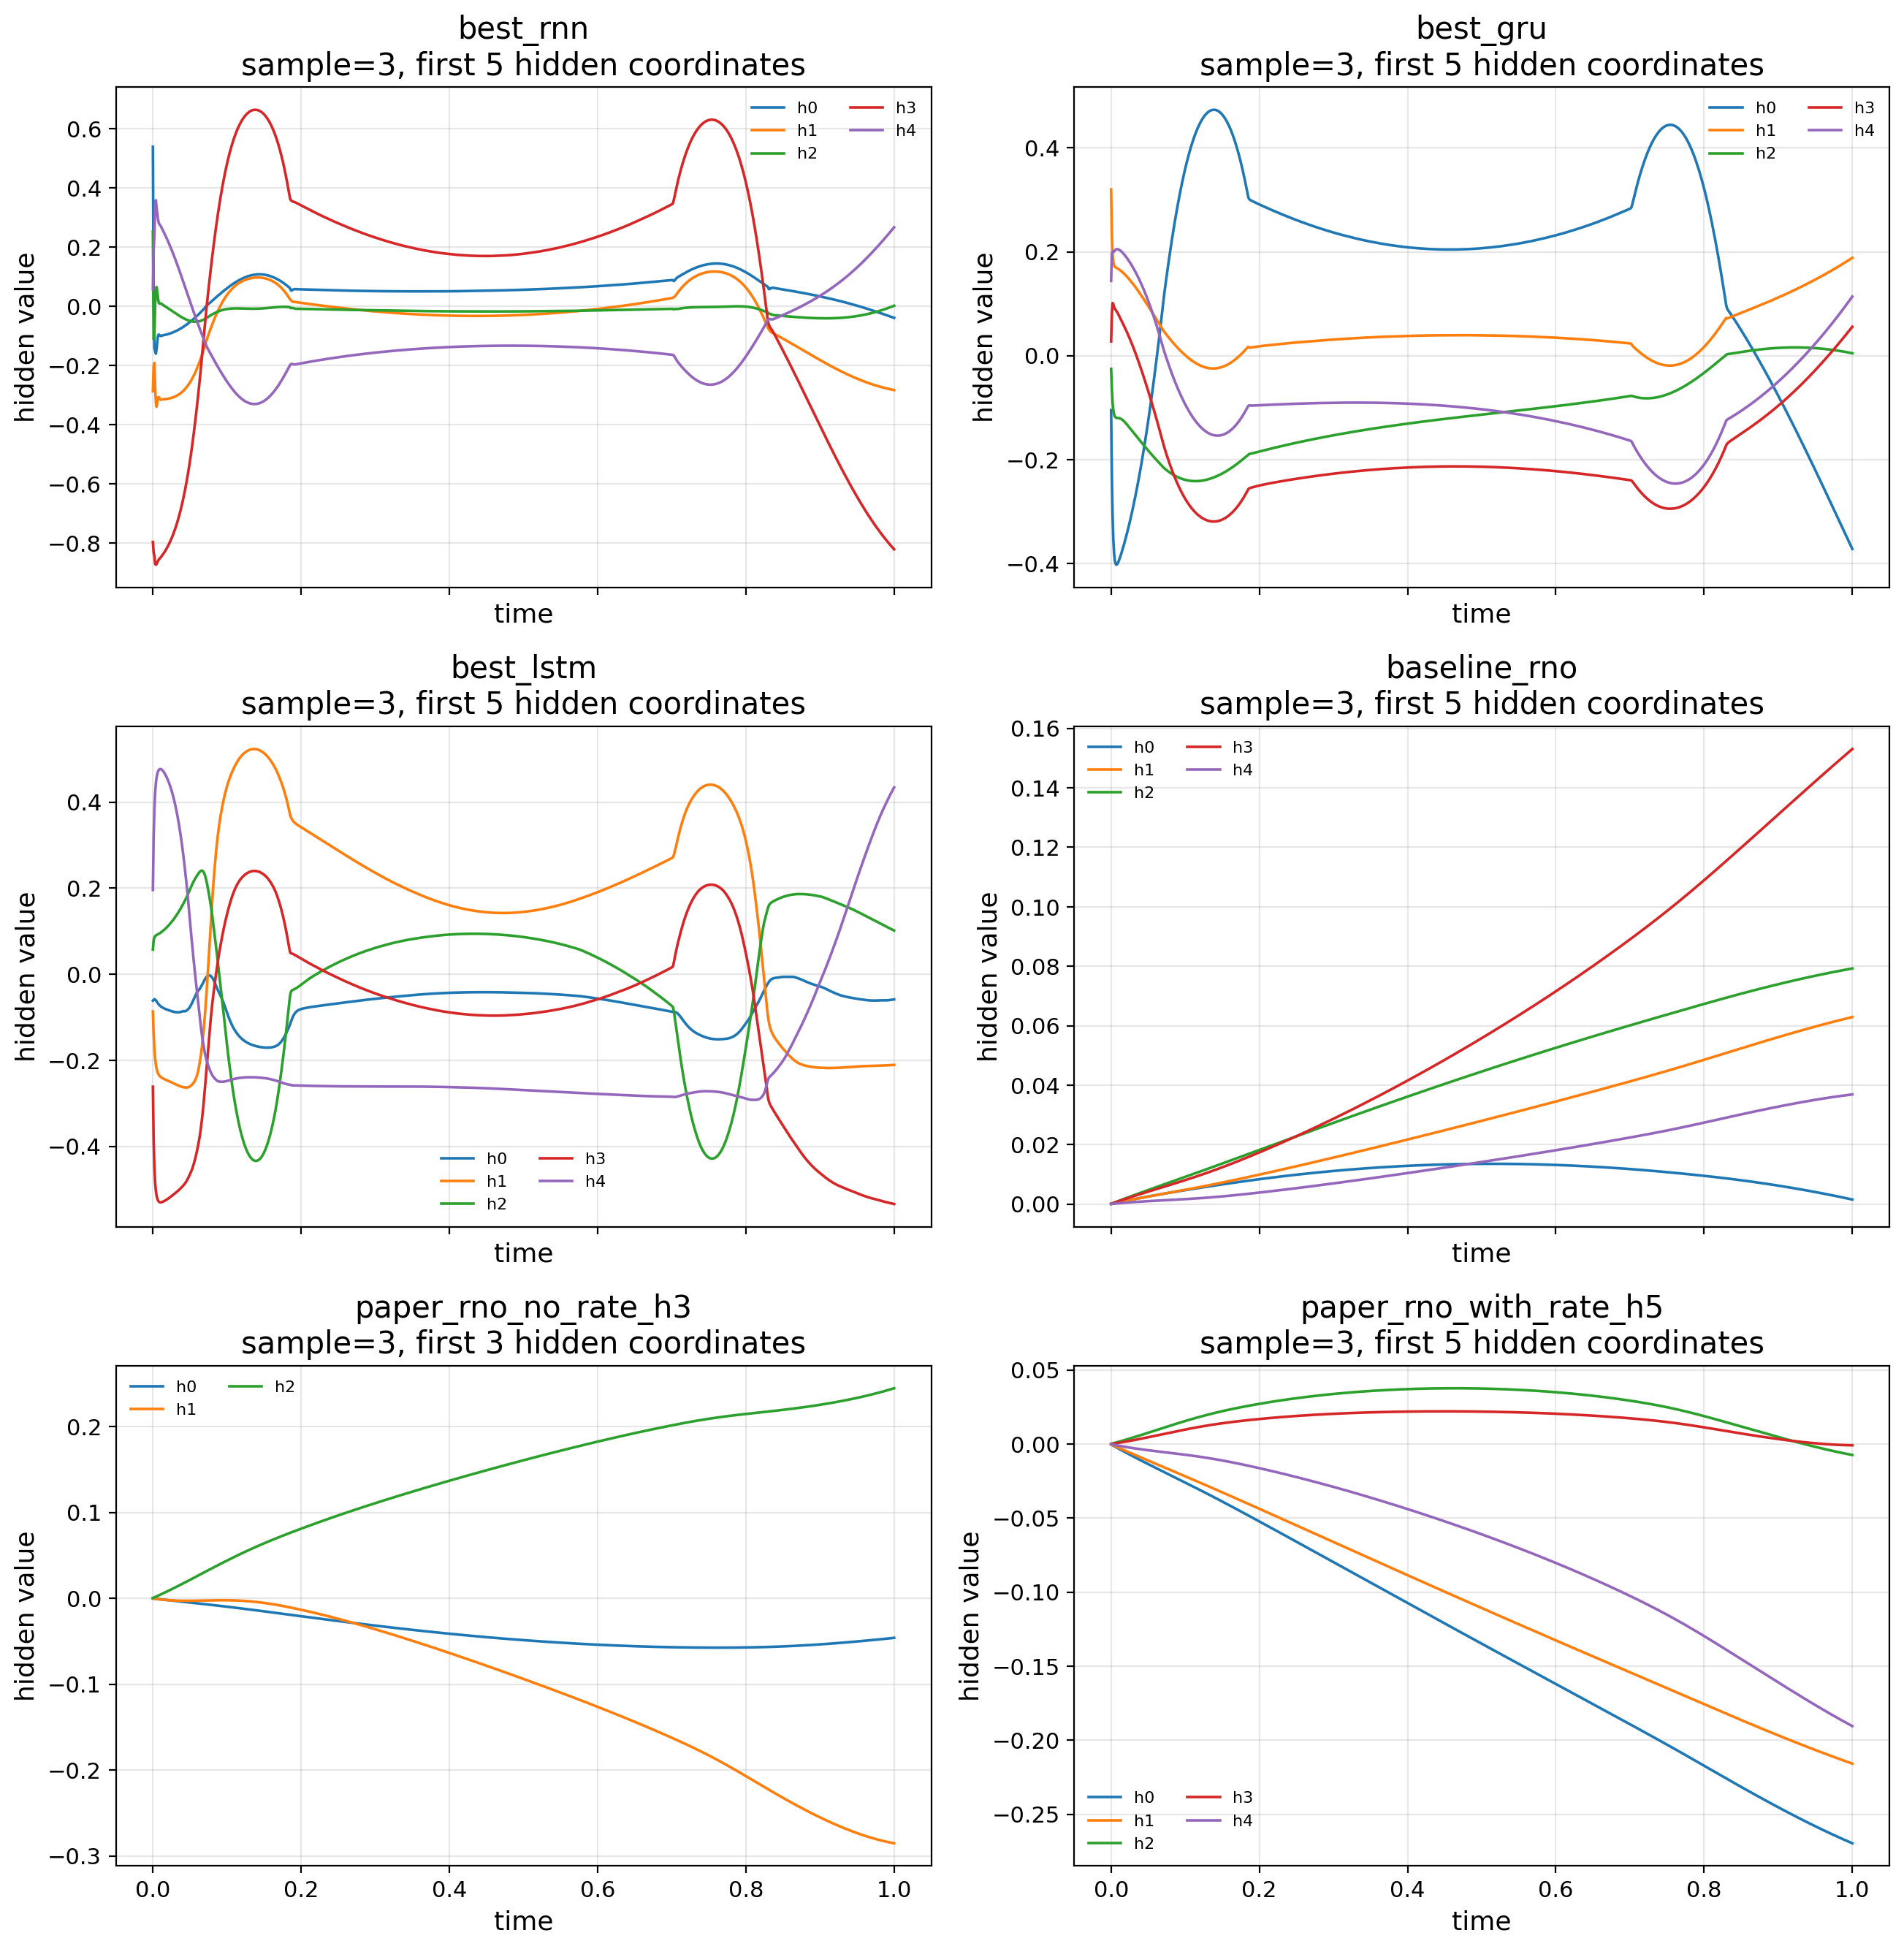
\includegraphics[width=\textwidth]{11_hidden_state_time_traces.png}
    \caption{Representative hidden coordinates as functions of time.}
\end{subfigure}
\hfill
\begin{subfigure}[h]{0.6\textwidth}
    \centering
    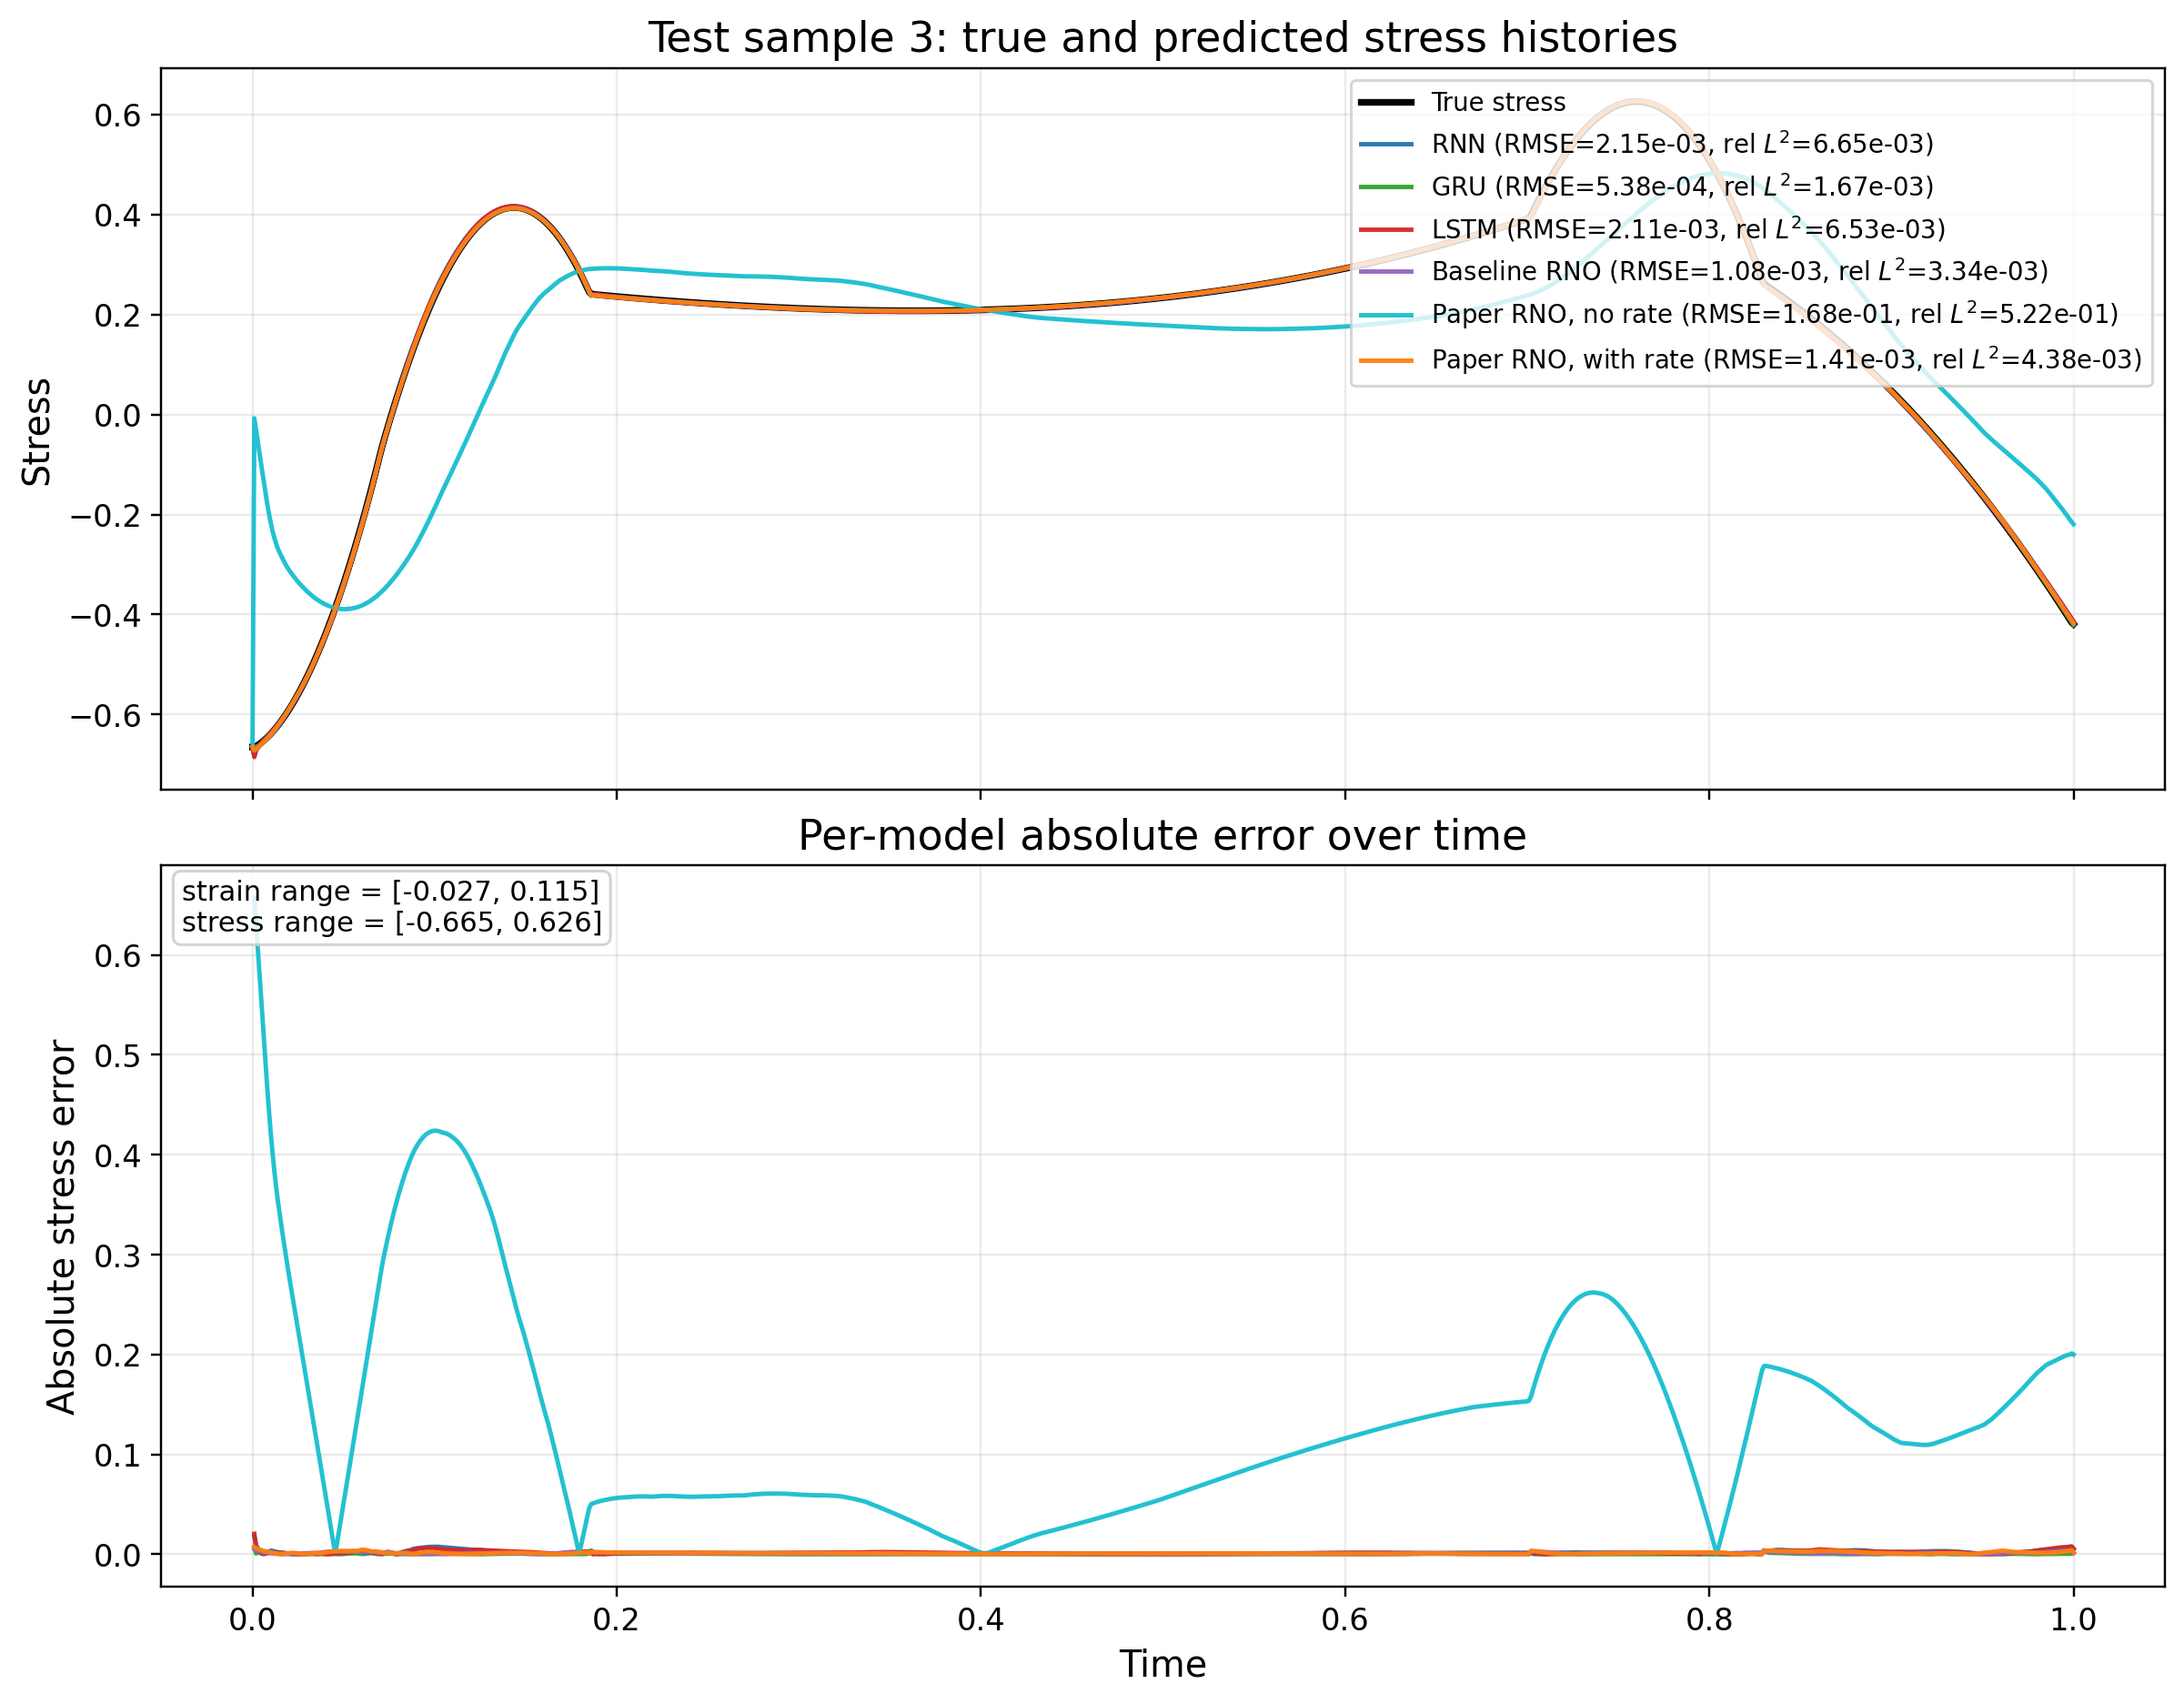
\includegraphics[width=\textwidth]{figures/sample_3_model_comparison.png}
    \caption{True and predicted stress histories for test sample 3 across the main models.}
\end{subfigure}
\caption{Hidden-state trajectories and overall trajectories comparisons.}
\label{fig:hidden_state_comparison}
\end{figure}

To understand why large hidden sizes can still behave as if only a few latent directions matter, the hidden-state trajectories were extracted and analysed by PCA. Figure~\ref{fig:hidden_state_geometry} shows the explained variance and correlation summaries. The main result is that the strongest models occupy a highly redundant latent space. The best GRU uses $40$ hidden channels, but the first two principal components already explain $99.21\%$ of the hidden-state variance. The baseline RNO is similar, with $99.14\%$ explained by the first two components. Even the paper RNO with rate and $h=5$ places $99.77\%$ of its variance in the first two components.

\begin{figure}[h]
\centering
\begin{subfigure}[h]{0.6\textwidth}
    \centering
    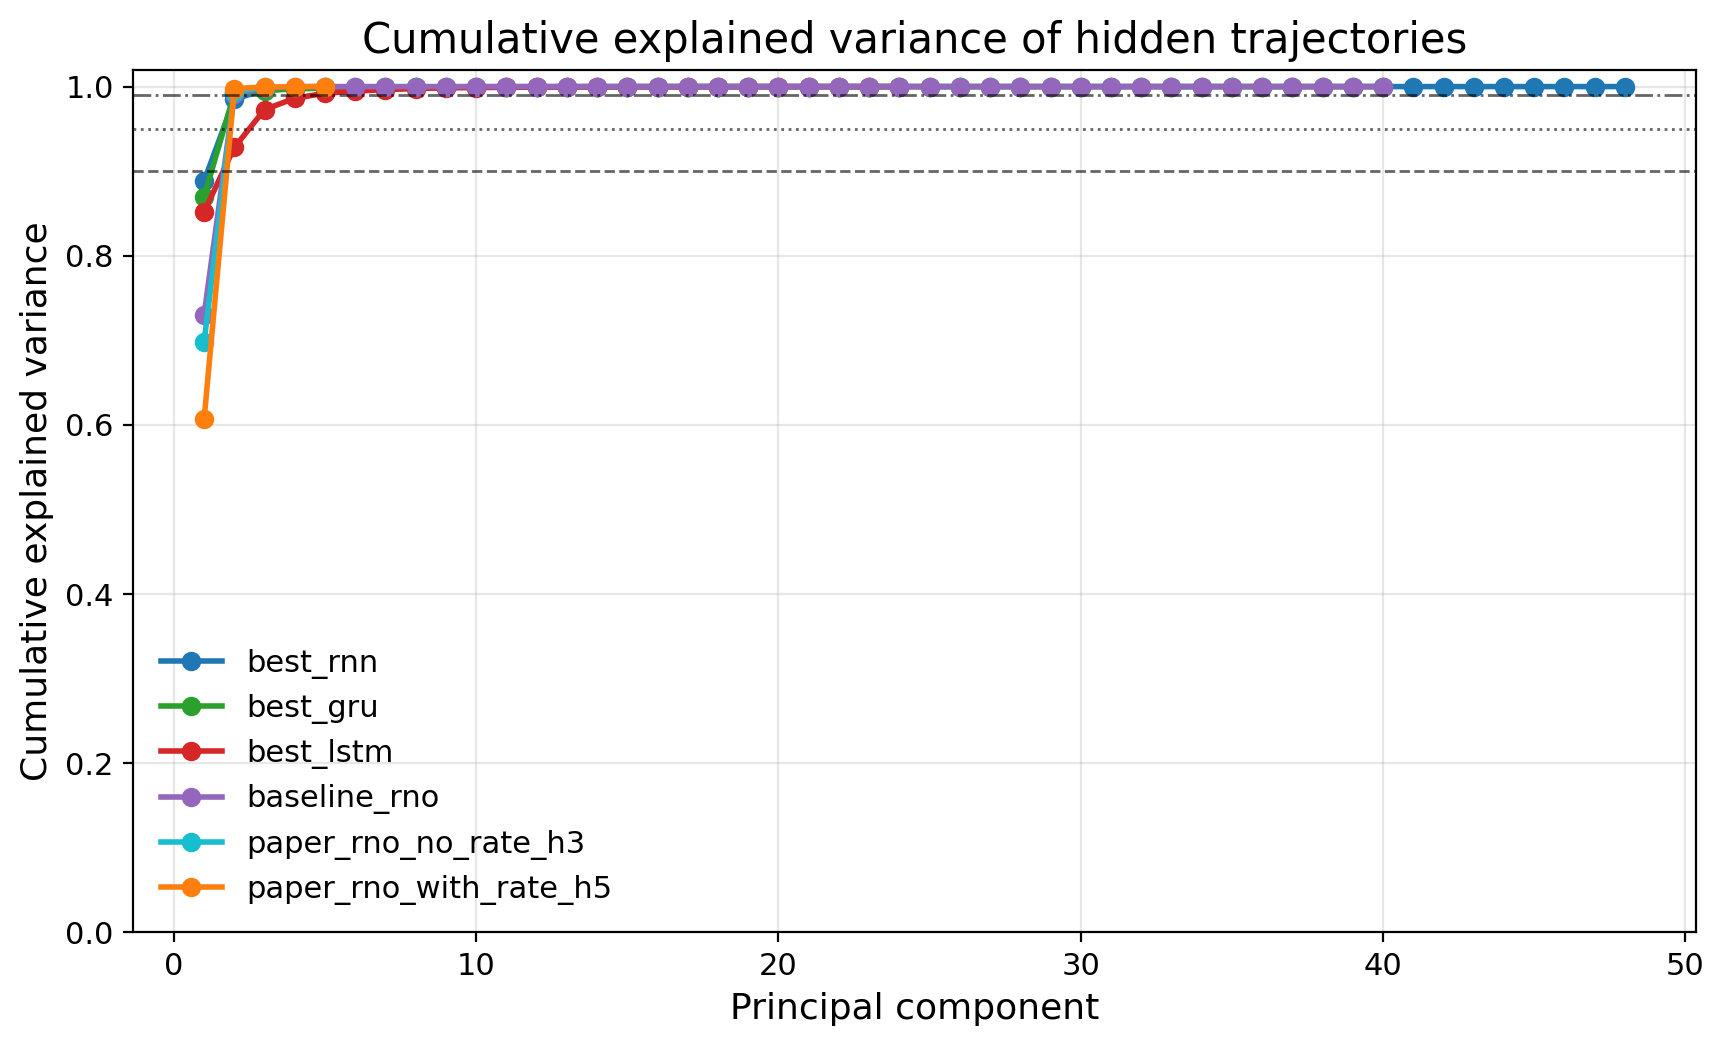
\includegraphics[width=\textwidth]{11_hidden_state_pca_explained_variance.png}
    \caption{PCA explained-variance curves for hidden trajectories.}
\end{subfigure}
\hfill
\begin{subfigure}[h]{0.6\textwidth}
    \centering
    
\includegraphics[width=\textwidth]{11_hidden_state_correlation_heatmaps.png}
    \caption{Hidden-state correlation heatmaps.}
\end{subfigure}
\caption{Hidden-state geometry for the trained models. High-performing models use latent spaces that are much more redundant than their raw hidden dimension suggests, with very strong pairwise correlations and very rapid PCA saturation.}
\label{fig:hidden_state_geometry}
\end{figure}

This observation helps explain the earlier threshold experiments. A large hidden size does not imply that the model is using all channels independently. In the cell-based models especially, many hidden channels collapse onto a low-dimensional manifold. That makes the mapping from ``hidden size'' to ``number of physical internal variables'' non-trivial. The dimensionality-reduction argument of Liu et al.~\cite{Liu_2023} is therefore useful as supporting evidence, but not as a standalone proof. Low latent dimensionality can coexist with both good and bad predictive performance. The paper-inspired no-rate model at $h=3$ is low dimensional, but is still much less accurate than the with-rate and GRU models because its constitutive inputs are more restricted.

\FloatBarrier

\subsection{Best inferred answer to lowest hidden variables required}

Taken together, these results suggest that the constitutive memory is low-dimensional, with the PCA analysis indicating that the learned latent trajectories of the strongest models are effectively two-dimensional. This is also consistent with a first-principles interpretation of the three-phase one-dimensional viscoelastic composite, for which only two independent internal variables are required once the observable macroscopic strain provides a compatibility constraint, as the third can be determined from the other two.



\FloatBarrier
\section{Conclusion}

This coursework addressed the constitutive-learning problem in multiple stages. 

\paragraph{(a)}First, the macroscopic constitutive input and output were defined as a strain-history-to-stress-history operator, mapping the applied macroscopic strain history to the corresponding macroscopic stress history. 

\paragraph{(b)}Second, recurrent neural operators based on vanilla RNN, GRU, and LSTM cells were designed, trained, and compared. Optuna hyperparameter optimisation showed that the GRU was the strongest predictive model on this dataset, achieving the lowest validation loss, the lowest test errors, and the most consistently accurate qualitative behaviour on held-out and unseen loading paths. The best GRU reached a validation loss of $8.36\times10^{-7}$ and a test relative $L^2$ error of $3.72\times10^{-3}$.

\paragraph{(c)}The third stage investigated the minimum number of hidden or internal variables required to represent the constitutive memory. A simple universal threshold did not emerge across all architectures. In the GRU and other rate-informed models, explicit access to current strain, previous strain, and strain rate makes the hidden state only part of the constitutive memory, so the hidden-dimension sweeps improve smoothly rather than exhibiting a sharp cliff. 

For this reason, more explicitly state-space models were introduced through the baseline RNO and the two paper-inspired forward-Euler RNO variants.

The clearest threshold-like result was obtained from the paper-inspired no-rate RNO, where the smallest hidden dimension within $5\%$ of the best validation loss was $h\approx 3$. However, this model was also substantially less accurate than the best GRU and the with-rate paper RNO, showing that interpretability was gained at the cost of predictive performance, and ultimately modelling the constitutive relation much weaker than the others. Once explicit strain rate was reintroduced, the paper-inspired model became much more accurate, and the dependence on hidden size became smooth again, indicating that rate information supplies a large fraction of the constitutive structure directly.

The hidden-state geometry analysis helped reconcile these observations. PCA and correlation analysis showed that the strongest models, despite having much larger nominal hidden sizes, evolve on highly redundant low-dimensional latent manifolds. In particular, the dominant hidden-state dynamics of the best models were effectively two-dimensional. This is consistent with a first-principles interpretation of the one-dimensional three-phase viscoelastic composite, for which only two independent internal variables are expected once the observable macroscopic strain provides a compatibility constraint.

The most defensible final answer to part~(c) is therefore that the constitutive memory is low-dimensional, of order two to three, rather than being associated with a single architecture-independent hidden size. Empirically, the strongest evidence came from the latent-state geometry and first-principles interpretation, suggesting an effective internal-variable dimension closer to $2$. Therefore, we can conclude that whilst we may not be able to identify one universal integer that applies to every recurrent architecture, we can show consistently that only a very small number of latent directions are needed to capture the macroscopic viscoelastic memory.

\bibliographystyle{unsrt}
\bibliography{references}


\includepdf[pages=-]{PDFs/SSD_new.pdf}

\end{document}
